\documentclass[psfig,preprint]{aastex}

\makeatletter
\renewcommand\theequation{\thesection.\arabic{equation}}
	\@addtoreset{equation}{section}
\renewcommand\thefigure{\thesection.\arabic{figure}}
	\@addtoreset{figure}{section}
\renewcommand\thetable{\thetable.\arabic{table}}
	\@addtoreset{table}{section}
\makeatother

\begin{document}

\setcounter{section}{-1}

\title{LEAST-SQUARES AND CHI-SQUARE FOR THE BUDDING AFICIONADO: \\ 
ART AND PRACTICE } 

\author{\copyright Carl Heiles \today }

	In our never-ending attempt to make your life easier, we present
you with this highly instructive, time-saving, and labor-saving
informative document! Here we give heuristic derivations, discussions,
examples, and the prescription for doing least-squares the easy way
using matrix techniques generally, and specifically in IDL.  This
prescription is given as an example in \S\ref{numexample},  and the {\it
power-user} can skip the details and go directly there.  

	This document is an update, correction, clarification, and
elaboration of a previous one made exclusively for the undergraduate lab
class. Here we extend the discussion considerably to cover most of what
anyone will need in future professional life. This makes the document
longer, but the first parts (\S \ref{sectionone} to
\ref{chauvenetsection}) are still accessible at the introductory level
because they haven't changed much. We occasionally refer to the books
Bevington and Robinson (1992; BR), Cowan (1998),  Press et al.\ (2001;
Numerical Recipes, NR) and Taylor (1997; T97), and we update the
notation to partially conform with NR. We owe sections
\ref{chauvenetsectiontwo} and \ref{medianfitting} to the 
excellent website of Stetson, {\it
http://nedwww.ipac.caltech.edu/level5/Stetson/Stetson4.html}.
Section \ref{bothsection} treats the case when all measured parameters
have errors; we use the very general approach of Jefferys  (1980).

	We begin with least-squares in the classic sense, meaning we
minimize the sum of squares instead of minimizing $\chi^2$.   In
astronomy,  more often than not you don't have an independent assessment
of the intrinsic uncertainty in the data, which means you cannot
evaluate $\chi^2$, and the least squares  approach is the only option.
However, often in astronomy you do want to weight observations
differently, e.g.\ because of integration time, and this requires an
approach similar to the $\chi^2$ one. In later sections we generalize to
the $\chi^2$ and this other weighted-observations case.

\tableofcontents

\section{LEAST-SQUAREs FITTING FOR TWO PARAMETERS, AS WITH A STRAIGHT
LINE.} \label{sectionone}

\subsection{The closed-form expressions for a straight-line fit}

	First consider the least-squares fit to a straight line.  Let
$y_m$ be the $m^{th}$ measurement of the observed quantity (in this
example, $y_m$ is zenith distance; $t_m$ be the time of the
$m^{th}$ measurement; $M$ = the total number of observations, i.e.\ $m$
runs from 0 to $M-1$.  Remember that in the least-squares technique,
quantities such as $t_m$ are regarded to be known with high accuracy
while the quantity $y_m$ has uncertainties in its measurement. 

	We expect the zenith distance $y_m$ to change linearly with
time as follows:

\begin{equation} \label{one}
A + B t_m = y_m \; .
\end{equation}

\noindent Given this, one does the maximum likelihood (ML) estimate assuming
Gaussian statistics. When all measurements have the same intrinsic
uncertainty, this is the same as looking for the solution that minimizes
the sum of the squares of the residuals (which we will define later). 
This leads to the pair of equations (Taylor 8.8, 8.9), called the {\it
normal equations}

\begin{mathletters} \label{normalone}
\begin{equation}
AN + B \ \sum t_m = \sum y_m
\end{equation}
\begin{equation}
A \ \sum t_m + B \ \sum t_m^2 = \sum t_m y_m \ .
\end{equation}
\end{mathletters}

\noindent Two equations and two unknowns---easy to solve! The
closed-form equations for $(A,B)$ are Taylor's equations 8.10 to 8.12.

\subsection{Better is the following generalized notation.}

	We want a way to generalize this approach to include any
functional dependence on $t$ and even other variables, and to have an
arbitrarily large number of unknown coefficients instead of just the two
$(A,B)$. This is very easy using matrix math.  We will ease into this
matrix technique gently, by first  carrying through an intermediate
stage of notation. 

	First generalize the straight-line fit slightly by having two
functional dependences instead of one. We have something other than the
time $t_m$; call it $s_m$. For example, we could have $s_m = \cos (t_m)$
or $s_m = t_m^2$; or we could have $s_m = x_m$, where $x_m$ is the
position from which the observation was taken. To correspond to equation
\ref{one}, $s_m = 1$. Then we rewrite equation \ref{one} to include this
extra dependence

\begin{equation} \label{two}
A s_m + B t_m = y_m \; .
\end{equation}

\noindent There are still only two unknown parameters, so this is an
almost trivial generalization; later we'll generalize to more
parameters.

	We have $M$ equations like equation \ref{two}, one for each
measurement.  They are known as the {\it equations of condition} because
they are the equations that specify the theoretical model to which we
are fitting the data. There are $M$ equations of condition and only two
unknowns ($A$ and $B$).  This is too many equations! We have to end up
with a system in which the number of equations is equal to the number of
unknowns.

	To accomplish this, from equation \ref{two} we form the {\it
normal equations}.  The number of normal equations is equal to the
number of unknowns, so in this case we will have two.   We could carry
through the same ML derivation to derive equations equivalent to
equation \ref{normalone}; the result is

\begin{mathletters} \label{ones}
\begin{equation}
A\ \sum s_m^2 + B \ \sum s_m t_m = \sum s_m y_m
\end{equation}
\begin{equation}
A \ \sum s_m t_m + B \ \sum t_m^2  = \sum t_m y_m \ .
\end{equation}
\end{mathletters}

\noindent We can rewrite these equations using the notation $[st] =
\sum s_m t_m$, etc.:

\begin{mathletters} \label{normaltwo}
\begin{equation}
A [ s^2 ] + B [ s t ] = [ s y ]
\end{equation}
\begin{equation}
A [ s t ] + B [ t^2 ] = [ t y ] \ .
\end{equation}
\end{mathletters}

\noindent This is, of course, precisely analogous to equation
\ref{normalone}. And now it's clear how to generalize to more
parameters!

\section{LEAST-SQUARES FITTING FOR MANY PARAMETERS, AS WITH A CUBIC}
\label{sectiontwo}

	With this notation it's easy to generalize to more ($N$)
unknowns: the method is obvious because in each equation of condition
(like equation \ref{two}) we simply add equivalent additional terms such
as $C u_m$, $D v_m$, etc; and in the normal equations (equation
\ref{normaltwo}) we have more products and also more normal equations. 

	Let's take an example with four unknowns ($N=4$), which we will
denote by $A, B, C, D$; this would be like fitting a cubic.  With $N=4$
we need at least five datapoints ($M=5$), so there must be at least
five equations of condition.  The generalization of equation \ref{ones}
is the $M$ equations

\begin{equation} \label{eqcond}
A s_m + B t_m + C u_m + D v_m = y_m \; ,
\end{equation}

\noindent with $m = 0 \rightarrow (M-1)$.  Again, the
least-squares-fitting process assumes that the $s_m, t_m, u_m, v_m$ are
known with zero uncertainty; all of the uncertainties are in the
measurements of $y_m$.  We then form the four normal equations; the
generalization of equation \ref{normaltwo} written in matrix format is:

\begin{eqnarray} \label{smeqn} 
\left[ 
\begin{array}{cccc} 
{[ ss ]} & {[ st ]} & {[ su ]} & {[ sv ]} \\ 
{[ ts ]} & {[ tt ]} & {[ tu ]} & {[ tv ]} \\ 
{[ us ]} & {[ ut ]} & {[ uu ]} & {[ uv ]} \\ 
{[ vs ]} & {[ vt ]} & {[ vu ]} & {[ vv ]} \\
\end{array} 
\; \right] 
\left[ 
\begin{array}{c} 
A \\ 
B \\ 
C \\ 
D \\
\end{array} 
\; \right] 
\; = 
\left[ 
\begin{array}{c} 
{[ s y ]} \\ 
{[ t y ]} \\ 
{[ u y ]} \\ 
{[ v y ]} \\ 
\end{array} 
\; \right]
\end{eqnarray} 

\noindent The $N \times N$ matrix on the left is symmetric. With $N$
equations and $N$ unknowns, you can actually {\it solve} for $A, B, C,
D$! 

\section{FAR, FAR BEST AND EASIEST: MATRIX ALGEBRA} \label{matrixmethod}

	The above equations are terribly cumbersome to solve in a
computer code because they require lots of loops.  However, it becomes
trivial if we use matrices.  Here we designate a {\bf matrix} by {\bf
boldface} type. 

	We illustrate the matrix method by carrying through the above
$N=4$ example, and we assume that there are 5 independent measurements
($M=5$).  We first define the matrices

\begin{mathletters} \label{matrixdefinition}
\begin{eqnarray} 
{\bf X} = \left[
\begin{array}{cccc} 
{s_0} & {t_0} & {u_0} & {v_0} \\ 
{s_1} & {t_1} & {u_1} & {v_1} \\ 
{s_2} & {t_2} & {u_2} & {v_2} \\ 
{s_3} & {t_3} & {u_3} & {v_3} \\
{s_4} & {t_4} & {u_4} & {v_4} \\
\end{array} 
\; \right] 
\end{eqnarray}
%\end{mathletters}

%\begin{mathletters}
\begin{eqnarray}
{\bf a} = \left[
\begin{array}{c}
A \\
B \\
C \\
D \\
\end{array} \; \right] 
\end{eqnarray}
%\end{mathletters}

%\begin{mathletters}
\begin{eqnarray}
{\bf Y} = \left[
\begin{array}{c} 
{y_0} \\ 
{y_1} \\ 
{y_2} \\ 
{y_3} \\ 
{y_4} \\ 
\end{array} 
\; \right]
\end{eqnarray} 
\end{mathletters} 

\noindent so, in matrix form, the equations of condition (equation
\ref{eqcond}) reduce to the single matrix equation

\begin{equation}
\label{equationofcondition}
{\bf X \cdot a} = {\bf Y} \; .
\end{equation}

\noindent The notation for these equations corresponds to NR's. We write
them with subscripts $\sigma$ to emphasize that they are calculated
without dividing by $\sigma_{meas}$, i.e.\ that we are doing least
squares instead of chi-square fitting. For chi-square fitting, see \S
\ref{chisqsection} and \ref{chicoeffs}.

	Our matrix $\mathbf{X}$ corresponds to NR's ``design
matrix'' $\bf A$ of Figure 15.4.1, except that our elements are not
divided by $\sigma_{meas,m}$, and the matrix equation of condition
(equation \ref{equationofcondition}) is identical to the expression
inside the square brackets of NR's equation 15.4.6. The differences
arise because here we are discussing least-squares fitting instead of
chi-square fitting, i.e.\ we have omitted the factors involving
$\sigma_{meas,m}$, the intrinsic measurement uncertainties (\S
\ref{chisqsection}).

	Again, there are more equations than unknowns so we can't solve
this matrix equation directly.  So next we form the normal equations
from these matrices.  In matrix form, the normal equations (equation
\ref{smeqn}) reduce to the single equation 

\begin{equation} \label{matrixnormal}
\mathbf{[\alpha] \cdot a} = \mathbf{[\beta]} \; ,
\end{equation}

\noindent (NR equation 15.4.10), where

\begin{mathletters} 
\label{ssdef}
\begin{equation} 
[\alpha] = {\bf X^T \cdot X} 
\end{equation}
\begin{equation}
[\beta] = {\bf X^T \cdot Y} \ .
\end{equation}
\end{mathletters}

\noindent The matrix $[\alpha]$ is known as the {\it curvature
matrix} because each element is twice the curvature of $\sigma^2$ (or
$\chi^2$) plotted against the corresponding product of variables. 

	The number of equations is equal to the number of unknowns, so
the solution of the matrix equation is easy---just rewrite it by
multiplying both sides by the inverse of $[\alpha]$ (that is, by
$[\alpha]^{-1})$, which gives

\begin{equation}
\label{adef}
{\bf a} = [\alpha]^{-1} \mathbf{ \cdot [\beta]} \; .
\end{equation}

\noindent All of these matrix operations are trivially easy in IDL (\S
\ref{numexample}). 

\section{UNCERTAINTIES IN THE DERIVED COEFFICIENTS} \label{sigmas}

	How about the uncertainties in the derived quantities contained
in the matrix ${\bf a}$?

       The first thing to do is derive the {\it sample} variance $s^2$
(the square of standard deviation, or mean error, or dispersion, etc) of
the individual datapoints using the generalization of the usual
definition for a straight average of $x$, $s^2 = [ \sum_0^{M-1} (x_m -
\overline{ x_m})^2/(M-1)]$.  The generalization is, simply, to replace   
the $M-1$ in the denominator by $\nu = M-N$.  In the straight-average
case, $N=1$ so this fits. Here $\nu$ is known as the number of {\it
degrees of freedom} and $N$, the number of unknown coefficients, is
known as the number of {\it constraints}. So we have

\begin{equation} \label{samplevarianceone}
s^2 = {1 \over M - N} \sum_{m=0}^{M-1} (y_m -
\overline{y_m})^2 \; ,
\end{equation}  

\noindent where $\overline{y_m}$ are the values for $y_m$ {\it
predicted by the derived quantities ${\bf a}$}. Note the difference:
$y_m$ are the {\it observed} values, while $\overline{y_m}$ are the
values {\it predicted by the least-squares fit}.  The predicted values
are those that are computed from the derived coefficients $A, B, C$\dots
The $M$ quantities

\begin{equation} \label{sequation}
\delta y_m = y_m - \overline{y_m}
\end{equation}

\noindent are called the {\it residuals} or {\it deviations} from the
fit.

        It's worth reiterating some essentials about $s^2$, and in
particular the denominator $(M-N)$.  First consider the case of a
single-parameter fit, e.g.\ $N=1$.  Then we cannot possibly derive a
sample variance from only one measurement $M=1$; but we can from two
$M=2$.  So the denominator makes sense from that standpoint.  The same
goes for $N>1$. 

        Next consider the effect of using $(M-N)$ in the denominator: it
increases $s^2$ by the ratio ${M \over M-N}$ over what you'd get if you
just took a straight average and used $M$. This compensates for the fact
that you are subtracting $\overline {y_m}$, which is derived from
the data, instead of the {\it truly} correct value $y^*$. (In
formal statistical language, $y^*$ is the mean of the parent
population from which your set of measurements is drawn.) If you used
the truly correct value $y^*$, then the sum would be larger than
when using $\overline{ y_m}$. The use of $M-N$ in the denominator
compensates for this larger value in exactly the right way: the
expectation value $E_{(s^2)}$ for a large number of experiments is
precisely equal to the normal variance $\sigma^2$, which you'd get by
using [$y^*$ and $M$] instead of [$\overline{y_m}$ and
$(M-N)$] in equation \ref{sequation}; see Cowan equations 5.9 and 5.10.
So $s^2$ is, in fact, exactly the number  we want: an unbiased estimate
of the true variance of our sample. Why    not use [$y^*$ and $M$]
in equation \ref{sequation}? The reason is obvious: we don't know
$y^*$! (If we did, we wouldn't be doing this analysis!)

	It's easy to calculate the $\overline{y_m}$ with matrices.
First define the matrix ${\bf \overline{ Y}}$ that contains these
values:

\begin{eqnarray}
{\bf \overline{ Y}} = \left[
\begin{array}{c} 
\overline{y_0} \\ 
\overline{y_1} \\ 
\overline{y_2} \\ 
\overline{y_3} \\ 
\overline{y_4} \\ 
\end{array} 
\; \right]
\end{eqnarray} 

{\noindent} Calculating ${\bf \overline{ Y}}$ is simple:

\begin{equation} \label{ybardefinition}
{\bf \overline{ Y}} = {\bf  X \cdot a} \; . 
\end{equation}

\noindent Note that ${\bf X}$ is already defined (equation
\ref{matrixdefinition}) and ${\bf a}$ was solved for in equation
\ref{adef}. It's convenient to define the residual matrix

\begin{equation}
{\bf \delta Y } = {\bf Y - \overline{ Y}}
\end{equation}

\noindent so we can write

\begin{equation} \label{samplevariancetwo}
s^2 = {1 \over M - N} {\bf \delta Y^T \cdot \delta Y} \; . 
\end{equation}

	This is the sample variance of the datapoints, not the variances
in the derived coefficients. We can obtain these as before, by
generalizing the results from the two-parameter case like the
straight-line fit discussed in \S \ref{sectionone}. We won't go through
the derivation here; you can find it in Taylor \S 8.4 and equation 8.16,
8.17. The result is

\begin{equation} \label{coeffvarianceone}
{\bf s_a}^2 = s^2 diag \{[\alpha]^{-1} \} \ .
\end{equation}

\noindent Or, to put it simply in words: to get the variance of 
coefficient $n$ in the matrix ${\bf a}$, multiply $s^2$ by the $n^{th}$
diagonal element of $[\alpha]^{-1}$. 

	Although the above equation for ${\bf s_a}^2$ is correct, there
is more to the story because of covariances, which are the off-diagonal
elements. We return to this topic in \S \ref{ncov} and \S \ref{chicoeffs}. 

\section{A NUMERICAL EXAMPLE AND ITS SOLUTION IN IDL} \label{numexample}

	If the following sounds like Greek to you, take a look at \S
\ref{matrixmethod} and \ref{sigmas}.

\subsection{Generation of the numerical example}

	Suppose that we make four measurements of the angle $y$ and
we want to fit to a parabolic function in time $t$.  In the notation of
equation~\ref{eqcond}, $s$ would be unity, $t$ the time, and $u$ the
time squared, so the number of unknowns is three ($N=3$).  Because there
are four independent measurements ($M=4$) the subscripts run from $m = 0
\rightarrow 3$.  Suppose that the four values of time are 5, 7, 9, 11. 

\begin{figure}[h!]
\begin{center}
\leavevmode
%\includegraphics[height=7.5in, width=6.0in]{twolvl3b.ps}
\includegraphics[scale=.55, angle=90]{lsfitfig.ps}
%\includegraphics{twolvla.ps}
\end{center}
\caption{Our numerical example. Stars are the four datapoints; the solid
line is the fit. We perform two fits: one uses the original definition
of time; the other uses $(time-8)$, in effect moving the $y$-axis to the
dashed line. The two fits give the same line but the coefficients and
their errors differ greatly.\label{lsfitfig}}
\end{figure}

	First we create the matrix {\bf X} in IDL

\begin{equation}
{\bf X = fltarr(N,M) = fltarr(3,4)}
\end{equation}
	
\noindent and then we populate it with numbers.  In your own work, you
would normally do this by reading a data file and transferring the
numbers to the matrix using IDL commands; to work through this example,
you might manually type them in.  After populating the matrix, in direct
correspondence with equation \ref{matrixdefinition}a we have $s_m = 1$,
$t_m = time_m$, $u_m = time_m^2$:

\begin{mathletters}
\begin{eqnarray}
{\bf X} = \left[
\begin{array}{ccc}
1  &  5   &  25  \\
1  &  7   &  49  \\
1  &  9   &  81  \\
1  &  11  &  121 \\
\end{array} \; \right] \ .
\end{eqnarray}
\end{mathletters}

\noindent Suppose that the four measured values of $y$ are
(equation~\ref{matrixdefinition}c)

\begin{mathletters}
\begin{eqnarray}
{\bf Y} = \left[
\begin{array}{c}
142 \\
168 \\
211 \\
251 \\
\end{array} \; \right] \; .
\end{eqnarray}
\end{mathletters}

\noindent Figure \ref{lsfitfig} shows the datapoints, together with the
fitted curve.

	One word of caution here: in IDL, to get these into a column
matrix, which is how we've treated $\bf Y$ above, you have to define
${\bf Y}$ as a two-dimensional array because the second dimension
represents the column. When working in IDL it's more convenient to 
define a row vector, which has only one dimension; in IDL you do this 
by defining ${\bf Y} = [142,168,211,251]$; you can make it into the
necessary column vector by taking its transpose, i.e.\ ${\bf Y =
transpose(Y)}$. 

	
\subsection{Solution of the Numerical Example in IDL} \label{idlsolution}

	In IDL we calculate the normal equation matrices and denote the
$[\alpha]$ in equation \ref{ssdef}a by ${\bf XX}$:

\begin{mathletters} \label{eqn24}
\begin{equation}
{\bf XX} = {\bf transpose(X) \# \# X} \; ,
\end{equation}

\noindent and we denote the $[\beta]$ in equation \ref{ssdef}b by {\bf
XY}:

\begin{equation}
{\bf XY} = {\bf transpose(X) \# \# Y} \; .
\end{equation}
\end{mathletters}

\noindent In IDL we take the inverse of $[\alpha]$ (same as $\bf XX$) by

\begin{equation}
{\bf XXI} = {\bf invert(XX)} \; .
\end{equation}

	The least-squares fitted quantities are in the matrix {\bf a}
(equation \ref{adef}), which we obtain in IDL with

\begin{equation}
{\bf a} = {\bf XXI \ \#\# \ XY} \; .
\end{equation}

	In IDL we denote the matrix of predicted values $\overline{
y_m}$ by ${\bf YBAR}$, which is 

\begin{equation}
\label{bteqn}
{\bf YBAR} = {\bf X \ \#\# \ a} \; ,
\end{equation}

\noindent and we can also define the residuals in $\bf Y$ as

\begin{equation}
{\bf DELY} = {\bf Y - YBAR} \ .
\end{equation}

\noindent In IDL we denote $s^2$ in equations \ref{samplevarianceone}
and \ref{samplevariancetwo} by $s\_sq$ and write 

\begin{mathletters}
\label{sigsq}
\begin{equation}
s\_sq = {\bf transpose(DELY) \#\# DELY}/(M-N) \; ,
\end{equation}

\noindent or

\begin{equation}
s\_sq = total({ \bf DELY} \wedge 2)/(M-N) \; . 
\end{equation}
\end{mathletters}

\noindent It is {\it always} a good idea to plot all three quantities
(the measured values {\bf Y}, the fitted values {\bf YBAR}, and the
residuals ${\bf DELY}$) to make sure your fit looks reasonable and to
check for bad datapoints. 

	To get the error in the derived coefficients we need a way to
select the diagonal elements of a matrix. Obviously, any $N \times N$
matrix has $N$ diagonal elements; a convenient way to get them is

\begin{equation}
diag \ elements \ of \ {\bf XXI}= {\bf XXI[(N+1) * indgen(N)]} \ .
\end{equation}

\noindent In IDL, we define the variances of
the $N$ derived coefficients by {\bf vardc} (think of ``{\bf var}iances of
{\bf d}erived {\bf c}oefficients''). You can get this as in equation
\ref{coeffvarianceone} from\footnote{If you used equation \ref{sigsq}a
instead of \ref{sigsq}b, then IDL considers $s\_ sq$ an array and you
need to use a $\#$ instead of a $*$ in this equation.}

\begin{equation} \label{lscoefferrorone}
{\bf vardc} = s\_sq * {\bf XXI[(N+1)*indgen(N)]} \; .
\end{equation}

\subsection {Discussion of the numerical example}

	For this numerical example, the solution (the array of derived
coefficients) is

\begin{mathletters}
\label{avalues}
\begin{eqnarray}
{\bf a} = \left[
\begin{array}{c}
96.6250 \\
4.5000 \\
0.8750 \\
\end{array} \; \right] 
\end{eqnarray}

\noindent and the errors in the derived coefficients [the square root of
the $\sigma^2$'s of the derived coefficients, i.e.  $[\sigma_n^2]^{1/2}$
or, in IDL, $sqrt({\bf vardc})$ in equations \ref{lscoefferrorone}] are:

\begin{eqnarray}
{\bf \sigma_A} = \left[
\begin{array}{c}
34.012 \\
9.000 \\
0.5590 \\
\end{array} \; \right] \; .
\end{eqnarray}
\end{mathletters}

\noindent These results look {\it horrible}: the uncertainties are large
fractions of the derived coefficients, 

	The reason: we have specifically chosen an example with terrible
covariance. And the great thing is this can be fixed easily (at least in
this case---certainly not always), without taking more data! 

\section{THE COVARIANCE MATRIX AND ITS NORMALIZED COUNTERPART} 
\label{ncov}

	First we provide a general discussion, then we apply it to the
above numerical example.

\subsection{ Definition of the normalized covariance (or correlation) matrix}

	The variances in the derived coefficients are obtained from the
diagonal elements of ${\bf XXI}$. The off-diagonal elements represent
the {\it covariances} between the derived coefficients. Covariance
means, specifically, the degree to which the {\it uncertainty} in {\it
one} derived coefficient affects the uncertainty in {\it another}
derived coefficient. 

	Because the covariance matrix elements relate pairwise to the
various coefficients, the units of the matrix elements are all
different. This makes it convenient to reduce all the matrix elements to
a standard set of units---namely, no units at all. So before discussing
the covariance matrix {\it per se}, we first discuss its normalized
counterpart. 

	The normalized covariance
matrix\footnote{It is a pleasure to thank Doug Finkbeiner for
introducing me to this concept.} {\bf ncov} is derived from ${\bf XXI}$
by dividing each element by the square root of the product of the
corresponding diagonal elements. Let ${\bf ncov}$ be the normalized
covariance matrix; then

\begin{equation}
ncov_{ik} = {XXI_{ik} \over \sqrt {XXI_{ii} \ XXI_{kk}}} \ .
\end{equation}

\noindent This is the same normalization that one does with the Pearson
linear correlation coefficient of two variables.  In fact, the elements
of the normalized covariance matrix {\it are} the correlation
coefficients.  So it makes sense to call this matrix the {\it
correlation matrix}, and many people do. In IDL, you do the following:
 
\begin{mathletters} \label{idlcovariance}
\begin{equation}
{\bf dc = XXI[(N+1)*indgen(N)]}
\end{equation}
\begin{equation}
{\bf ncov = XXI/{\it sqrt}(dc \# \#dc)} \ .
\end{equation}
\end{mathletters}

\noindent In the above, ${\bf dc \# \# dc}$ is an $N \times N$ matrix
consisting of products of the diagonals of ${\bf XXI}$, so dividing
${\bf XXI}$ by $sqrt({\bf dc \# \# dc})$ generates the normalized version. 

	Because {\bf ncov} is a {\it normalized} covariance matrix, you
might think that its non-normalized parent is {\bf XXI}---and you'd be
{\it almost} right.  For the least-squares case we are discussing, the
true covariance matrix ${\bf C}$ is\footnote{For chi-square, you use
$\sigma_{meas}^2$ instead of $s^2$; see \S \ref{chisqsection}.}

\begin{equation}
{\bf C} = s^2 \ {\bf XXI} \ .
\end{equation}

	In ${\bf ncov}$, the diagonal elements are all unity and the
off-diagonal elements reflect the interdependence of the derived
coefficients on each other.  The off-diagonal elements can range from
$-1 \rightarrow 1$. Each matrix element is the correlation coefficient
between the {\it uncertainties} of its two parameters. In particular,
suppose that the data happen to produce a coefficient that differs from
its true value by some positive number. If the normalized matrix element
is negative, then the other coefficient will tend to differ from its
true value by a negative number. 

	Here's a more detailed discussion of what the covariance means. 
Suppose you are least-squares fitting for two derived coefficients
($A_0$ and $A_1$).  When you do a least-squares fit to a set of data,
you are fitting one set of data out of a possible infinity of possible
sets that you'd get by repeating the experiment, and your particular set
of data happens to produce specific values of $\overline{ A_0}$ and $\overline{
A_1}$, which differ from the {\it true} values $(A_0^*, A_1^*)$ by
amounts $\delta A_0$ and $\delta A_1$.  If their covariance is zero,
then in the infinity of data sets you'd find that $\delta A_0$ is
uncorrelated with $\delta A_1$.  But if it is nonzero, these two
quantities would be correlated. 

	A high covariance is bad because the derived variables depend on
each other.  For one, this means that with noisy data power can be
shared or passed from one parameter to/from its covariant
counterpart(s). As we shall see in \S \ref{chicoeffs}, it also
significantly  influences the uncertainties in derived coefficients.
Often a high covariance results from a poor choice of functions that you
are fitting or even a bad choice of the zero point of the independent
variable---as in our numerical example (see the next subsection).  And,
as in that example, you can sometimes eliminate the bad covariance by
reformulating the problem---you don't even need to take more data! The
best reformulation involves using a set of orthonormal functions.
However, sometimes your interest is a specific set of functions that are
{\it not} orthogonal, and in such cases it makes no sense to convert to
orthogonal functions---because you just have to convert back again and
do the error propagation after-the-fact instead of letting the
least-squares process do it for you.

\subsection{ The covariance in our numerical example} \label{covarianceone}

	Apply equation \ref{idlcovariance} to obtain the covariance
matrix for our numerical example:

\begin{eqnarray}
{\bf ncov} = \left[
\begin{array}{ccc}
1  &  -.989848   &  .969717  \\
-.989848  &  1   &  -.993808  \\
.969717  & -.993808 &  1  \\
\end{array} \; \right] \; .
\end{eqnarray}

	The off-diagonal elements are {\it huge}.  This is the reason
why our derived coefficients have such large uncertainties.  Note,
however, that the fitted predicted fit is a good fit even with these
large uncertaintis. 

	In this seemingly innocuous example we have an excellent case of
a poor choice of zero point for the independent variable (the time). 
The reason is clear upon a bit of reflection. We are fitting for $y =
A_0 + A_1 t + A_2 t^2$. The coefficient $A_0$ is the $y$-intercept and
$A_1$ is the slope. Inspection of Figure \ref{lsfitfig} makes it very
clear that an error in the slope has a big effect on the $y$-intercept. 

	Now we retry the example, making the zero point of the time
equal to the mean of all the times, that is we set $(time_m = time_m -
8)$. We get the same fitted line, but the derived coefficients are
completely different---and amazingly better! We get

\begin{mathletters}
\begin{eqnarray}
{\bf A} = \left[
\begin{array}{c}
188.625 \\
18.500 \\
0.87500 \\
\end{array} \; \right] 
\end{eqnarray}

\begin{eqnarray}
{\bf \sigma_A} = \left[
\begin{array}{c}
3.58 \\
1.00 \\
0.559 \\
\end{array} \; \right] \; .
\end{eqnarray}
\end{mathletters}

\noindent In redefining the origin of the independent variable, we have
made the zero intercept completely independent of the slope: changing
the slope has no affect at all on the intercept. You can see this from
the normalized covariance matrix, which has become

\begin{eqnarray}
{\bf ncov} = \left[
\begin{array}{ccc}
1  &     0       &   -0.78086881  \\
   0  &  1   &    0  \\
 -0.78086881 &  0  &  1  \\
\end{array} \; \right] \; ,
\end{eqnarray}

\noindent which is nice, but not perfect: Our step is {\it partial}
because the second-order coefficient $A_2$ affects $A_0$ because, over
the range of $[(time - 8) = -3 \rightarrow +3]$, the quantity $[A_2 \;
\Sigma(time_m -8)^2]$ is always positive and is thereby correlated with
$A_0$.

	We could complete the process of orthogonalization by following
the prescription in BR chapter 7.3, which discusses the general
technique of orthogonalizing the functions in least-squares fitting. The
general case is a royal pain, analytically speaking, so much so that we
won't even carry it through for our example. But for numerical work you
accomplish the orthogonalization using Singular Value Decomposition
(SVD), which is of course trivial in IDL (\S \ref{SVD}).

	For some particular cases, standard pre-defined functions are
orthogonal. For example, if $t_m$ is a set of uniformly spaced points
between $(-1 \rightarrow 1)$ and you are fitting a polynomial, then the
appropriate orthogonal set is Legendre polynomials. This is good if your
only goal is to represent a bunch of points by a polynomial function,
because the coefficients of low-order polynomials are independent of the
higher ones. However, it's more work and, moreover, often you are
interested in the coefficients for specific functions that don't happen
to be orthogonal; in such cases, you should just forge ahead. 

	But {\it always} look at the normalized covariance matrix.
Suppose one pair of off-diagonal elements departs significantly from
zero. Then their corresponding functions are far from being orthogonal
and the variances of the derived coefficients will suffer as a result.
You might be able to eliminate one of the parameters to make the fit
more robust. For example, suppose one function is $t \cos (t)$ and the
other is $\sin(t) \cos (t)$. If the range of $t$ is small, these two
functions are indistinguishable and have a large covariance; you should
eliminate one from the fit. If the range of $t$ is large, there is no
problem.

	For further discussion of covariance, see \S \ref {chicoeffs}.
Also, you might also want to try out another example in Taylor's \S 8.5.

\section{REJECTING BAD DATAPOINTS I.: CHAUVENET'S CRITERION}
\label{chauvenetsection}

	Least-squares fitting is derived from the maximum likelihood
argument assuming the datapoint residuals $\delta y_m$ have a Gaussian
pdf. This means that the errors are distributed as 

\begin{equation}
p_{(\delta y; \sigma)} = {1 \over \sqrt{2\pi} \sigma} 
    e^{-\left( \delta y^2 \over 2 \sigma^2 \right)} \ ,
\end{equation}

\noindent where $\sigma^2$ is the true variance of the datapoints, i.e.\
$s^2$ in equation \ref{samplevarianceone} (to be precise, $s^2$ needs to
be averaged over many experiments). 

	More importantly, the probability of finding datapoints inside
the limits $\pm \Delta y$ is 

\begin{equation}
P_{(|\delta y| < \Delta y)} = \int_{-\Delta y}^{+\Delta y} 
  p_{(\delta y; \sigma)} d(\delta y) = 
  {\rm erf}\left({\Delta y \over \sqrt{2} \sigma} \right) \ ,
\end{equation}

\noindent where we use the commonly-defined error function ${\rm
erf}(X) = {1 \over \sqrt{\pi}} \int_{-X}^{+X} e^{-x^2} dx$. A
particularly important value is for $\Delta y = \sigma$, for which 

\begin{equation}
P_{(|\delta y| < \sigma)} = 0.683 \ .
\end{equation}

	If we have an experiment with $M$ datapoints, then the number of
datapoints we expect to lie outside the interval $\pm \Delta y$ is

\begin{equation}
M_{(outside \ \Delta y)} = M \left[ 1 - 
  {\rm erf} \left({\Delta y \over \sqrt{2} \sigma} \right) \right] \ .
\end{equation}

\noindent Chauvenet's criterion simply says: \begin{enumerate}

	\item Find $\Delta y$ such that $M_{(outside \ \Delta y)} =
0.5$. This is given by 

\begin{equation} \label{chauvenetexplicit}
{\Delta y \over \sigma} = \sqrt{2} \ {\rm erf}^{-1}\left( {1 - {1 \over 2M}} \right) \ .
\end{equation}

\noindent This criterion leads to the numbers in the associated table, 
which is a moderately interesting set of numbers. Many
astronomers adopt $3 \sigma$, which is clearly inappropriate for large
$N$! 

\begin{table} [!h]
\begin{center}
%\hline
%\caption{ Chauvenet's criterion versus $M$} \label{chauvenettable}
\begin{tabular}{cc} 
%\hline
\\ \hline \hline
\multicolumn{2}{c}{ Chauvenet's criterion versus $M$} 
\\ \hline
$M$ & $\Delta y \over \sigma$ \\ \hline
100 & 2.81 \\
1000 & 3.48 \\
$10^4$ & 4.06 \\
$10^5$ & 4.56 \\ \hline
\hline
\end{tabular}
\end{center}
\end{table}

 
	\item Discard all datapoints outside this range.

\end{enumerate}

	We offer the following important {\it Comments}:
\begin{itemize}

	\item This assumes data are Gaussian-distributed. In real life
this doesn't often happen because of ``glitches''. Examples of glitches
can be interference in radio astronomy, meteors in optical astronomy,
and cosmic rays on CCD chips. These glitches produce bad points that
depart from Gaussian statistics. They are often called {\it outliers}.

	It is very important to get rid of the outliers because the
least-squares process minimizes the {\it squares} of the residuals.
Outliers, being the points with the largest residuals, have a
disproportionately evil effect on the result.

	On the other hand, if your data don't follow Gaussian statistics
as their {\it intrinsic} pdf, then you should think twice before using
least squares! (Like, maybe you should try the median fitting discussed in
\S \ref{medianfitting}.)

	\item You may wish to relax Chauvenet's criterion by {\it
increasing} the $\Delta x$ beyond which you discard points. This is
being conservative and, in the presence of some non-Gaussian statistics,
not a bad idea. But think about why you are doing this before you do it.
Maybe the intrinsic statistics aren't Gaussian?

	You should {\it never} make Chauvenet's criterion more stringent
by {\it decreasing} the $\Delta x$ beyond which you discard points. This
rule hardly needs elaboration: it means you are discarding datapoints
that follow the assumed pdf!

	\item Most statistics books (e.g. Taylor, BR) harp on the purity
aspect. One extreme: don't throw out any datum without examining it from all
aspects to see if discarding it is justified. The other extreme: apply
Chauvenet's criterion, but do it {\it only once} and certainly not
repeatedly.

	Being real-life astronomers, our approach is different. There
{\it do} exist outliers. They increase the calculated value of $\sigma$.
When you discard them, you are left with a more nearly perfect
approximation to Gaussian statistics and the new $\sigma$ calculated
therefrom will be smaller than when including the outliers. Because the
original $\sigma$ was too large, there may be points that should have
been discarded that weren't. So our approach is: repeatedly apply
Chauvenet's criterion until it converges. 

	If it doesn't converge, or if it discards an inordinately large
number of datapoints, you've got real problems and need to look at the
situation from a global perspective.

	\item Many observers use the $3\sigma$ criterion: discard any
points with residuals exceeding $3\sigma$. This is definitely {\it not}
a good idea: the limit $3\sigma$ is Chauvenet's criterion for $M=185$
datapoints. Very often $M$ exceeds this, often by a lot. 

	\item To apply Chauvenet's criterion it's most convenient to
calculate the inverse error function. For this, you have two choices.
One (for sissies like myself), you can use {\bf inverf.pro} from my area
$\sim$heiles/idl/gen . But the real he-man will want to learn about
using a root-finding algorithm such as Newton's method (NR \S 9.4 and
9.6) together with the error function; both procedures exist in IDL as
{\bf newton} and {\bf errorf}. You at least ought to skim lightly some
of NR's chapter 9 about root finding, because some day you'll need it.

\end{itemize}

\section{NONLINEAR LEAST SQUARES} \label{nonlinearls}

	The least-squares formulation requires that the data values
depend {\it linearly} on the unknown coefficients. For example, in
equation \ref{one}, the unknown coefficients $A$ and $B$ enter linearly.

	Suppose you have a nonlinear dependence, such as wanting to
solve for $A$ and $B$ with equations of condition that look like 

\begin{equation} \label{basicone}
\sin(A t_m) + B t_m = y_m \; .
\end{equation}

\noindent What do you do here? You linearize the process, using the
following procedure. 

	First, assume trial values for $A$ and $B$; call these $A_0$
and $B_0$. You should pick values that are close to the correct ones. In
our example you wouldn't need to do this for $B$, but it's easier to
treat all coefficients identically. These trial values produce {\it
predicted} values $y_{0,m}$:

\begin{equation} \label{trialone}
\sin(A_0 t_m) + B_0 t_m = y_{0,m} \; .
\end{equation}

\noindent Subtract equation \ref{trialone} from \ref{basicone}, and
express the differences as derivatives. Letting $\delta A = A - A_0$ and
$\delta B = B - B_0$, this gives

\begin{equation} \label{difference}
\delta A [t_m \cos(A_0 t_m)] + \delta B t_m = y_m - y_{0,m} \; .
\end{equation}

\noindent This is linear in $(\delta A, \delta B)$ so you can solve for
them using standard least squares. Increment the original guessed values
to calculate $A_{0,new}=A_0 + \delta A$ and $B_{0,new}=B_0 + \delta B$,
These won't be exact because higher derivatives (including cross
derivatives) come into play, so you need to use these new values to
repeat the process. This is an iterative procedure and you keep going
until the changes become ``small''. The generalization to an arbitrarily
large number of unknown coefficients is obvious.

	We now offer some cautionary and practical remarks.

	{\bf (0)} In linear least squares, the curvature and covariance
matrices are set by the values of the independent variable, which here
is denoted by $t$, and are independent of the datapoint values. Here,
the matrix elements change from one iteration to the next because they
depend on the guessed parameters, and sometimes they even depend on the
datapoint values. 

	{\bf (1) Multiple minima:} Nonlinear problems often have
multiple minima in $\sigma^2$. A classical case is fitting multiple
Gaussians to a spectral line profile. Gaussians are most definitely not
orthogonal functions and in some cases several solutions may give almost
comparably good values of $\sigma^2$, each one being a local minimum.
For example, for the case of two blended Gaussians, one can often fit
two narrow Gaussians  or the combination of a wide and narrow Gaussian,
the two fits giving almost equal $\sigma^2$. The lower of these is the
real minimum but, given the existence of systematic errors and such, not
necessarily the best solution. The best solution is often determined by
physical considerations; in this case, for example, you might have
physical reasons to fit a broad plus narrow Gaussian, so you'd choose
this one even if its $\sigma^2$ weren't the true minimum.

	{\bf (2) The Initial Guess:} When there are multiple minima,
the one to which the solution converges is influenced by your initial
guess. To fully understand the range of possible solutions, you should
try different initial guesses and see what happens. If the solutions
always converge to the same answer, then you can have some confidence
(but not {\it full} confidence) that the solution is unique.

	{\bf (3) Iterative stability:} If your initial guess is too far
from the true solution, then the existence of higher derivatives means
that the computed corrections can be too large and drive the iterative
solution into instability. It is often a good idea to multiply the
derived correction factors ($\delta A$ and $\delta B$ above) by a factor
${\cal F}$ less than unity, for example ${\cal F} = 0.5$ or 0.75. This
increases the number of iterations required for convergence but often
allows convergence instead of producing instability.

	{\bf (4) Convergence criteria:} How do you know when the
solution has converged? One way: for each iteration, calculate the
uncertainties in the derived coefficients. If the uncertainty exceeds
the correction, then you are getting close. An alternate way, which I
usually use: if the fractional correction (e.g.~$\delta A \over A_0$)
decreases below some threshold, say $1\%$, you're close (some
parameters, such as angles, need a threshold that is absolute instead of
fractional).  At this point, if you are using ${\cal F} \neq 1$, set
${\cal F} = 1$, do a few more iterations, and you're done. 

	{\bf (5) Numerical derivatives:} Sometimes the equations of
condition are so complicated that taking the derivatives, as in
obtaining equation \ref{difference}, is a huge job and subject to
mistakes. So you can take numerical derivatives instead of analytic
ones. Be careful, though; it's safest to use double precision and think
a bit about numerical accuracy; take a look at NR's section 5.7 on
evaluating numerical derivatives.

	{\bf (6) Canned nonlinear least squares (particularly
Levenberg-Marquardt, and various Gaussian fit routines):} Packages like
IDL offer canned nonlinear least squares routines.  They are designed to
work well for a wide range of different problems.  However, for the
specific problem at hand you can often do better by tailoring things
(such as the factor ${\cal F}$ and convergence criteria above).  A good
example is Gaussian fitting: IDL's fitting program doesn't converge for
multiple overlapping Gaussians, while for many of these cases the
program that I wrote myself works fine; and converseley, my program
doesn't work well for single Gaussians with a small number of
datapoints, in which case IDL's \verb$GAUSSFIT$ is much better..

	When convergence is slow or doesn't occur because your functions
are complicated, you might wish to try the Levenberg-Marquardt method
(NR \S 15.5); IDL function {\bf LMFIT}.  This technique involves
increasing the diagonal elements of the curvature matrix by a set of
suitably chosen factors; when you get close to the minimum, it resets
these factors to unity.  LM is the gold standard for nonlinear
least-squares fitting because it is supposed to converge faster than
other methods.  Because of its sterling reputation, many people think
it's the panacea.  How many times have I seen journal articles saying
that the LM method was used---as if that's all one needs to know---but
without saying anything about the important stuff, such as how parameter
space was explored to determine uniqueness of the solution! See the
discussion in NR.  I've done lots of nonlinear fits and have never had
to resort to any tactic other than the simple, straightforward
linearization process discussed above. 

	{\bf (7) Be careful and LOOK at the solution before accepting
it!} These nonlinear problems can produce surprising results, sometimes
completely meaningless results. Don't rely on them to be automatic or
foolproof!

        {\bf (8) Reformulate! (?)} Sometimes you can avoid all this by
reformulating the problem. There are two cases: the harmless case and
the not-so-harmless case.

        An example of the harmless case is fitting for the phase $\phi$
in the function $y = \cos( \theta + \phi)$.  This is definitely a
nonlinear fit! But its easy to reformulate it in a linear fit using the
usual trig identities to write $y = A \cos \theta - B \sin \theta$,
where ${B \over A} = \tan \phi$.  Solve for $(A,B)$ using linear least
squares, calculate $\phi$, and propagate the uncertainties. 

        An example of the not-so-harmless case is in NR's \S 15.4
example: fit for $(A,B)$ with equations of condition $y_m = A
e^{-Bx_m}$.  They suggest linearizing by rewriting as $\log (y_m) = C -
Bx_m$, solving for $(B,C)$, and deriving $A$ after-the-fact.  This is
not-so-harmless because you are applying a nonlinear function to the
{\it observed} values $y_m$; thus the associated errors
$\sigma_{meas,m}$ are {\it also} affected.  This means you have to do
weighted fitting, which is discussed in \S \ref{chisqsection} below. 
Suppose that $A=1$, your datapoints all have $\sigma_{meas,m} = 0.05$,
and the observed $y_m$ ranges from 0.05 to 1.  The datapoint with $y_m =
0.05$ has a manageable $\sigma_{meas_m}$, but what is the corresponding
value of $\sigma_{meas,m}$ for $\log y_m = \log 0.05$? It's ill-defined
and asymmetric about the central value.  Or even, God forbid, you have
an observed $y_m$ that's {\it negative}??? Even for $y_m$ not near zero,
you need to calculate new $\sigma_{meas,m}$ by error propagation; in
this case, you need to reassign $\sigma(\log y) = {d \log y \over dy}
\sigma(y) = {\sigma(y) \over y}$.  This is OK when $y_m$ is large enough
so that the linear approximation is accurate, but if not the converted
noise becomes non-Gaussian. 

	You should regard your datapoints as sacrosanct and never apply
any nonlinear function to them.

\section{CHI-SQUARE FITTING AND WEIGHTED FITTING: DISCUSSION IGNORING
COVARIANCE } \label{chisqsection}

	In least-squares fitting, the derived parameters minimize the sum of
squares of residuals as in equation \ref{samplevarianceone}, which we
repeat here:

$$ s^2 = {1 \over M - N} \sum_{m=0}^{M-1} \delta y_m^2 \, . $$

\noindent where the $m^{th}$ residual $\delta y_m = (y_m -
\overline{y_m})$.  Chi-square fitting is similar except for two
differences.  One, we divide each residual by its intrinsic measurement
error $\sigma_{meas,m}$; and two, we define $\chi^2$ as the sum

\begin{mathletters} \label{chisqdefinition}
\begin{equation}
 \chi^2 = \sum_{m=0}^{M-1} {\delta y_m^2
     \over \sigma_{meas,m}^2 } \; . 
\end{equation}

\noindent Along with $\chi^2$ goes the {\it reduced} chi square
$\widehat{\chi^2} = {\chi^2 \over M-N}$

\begin{equation}
\widehat{\chi^2} = {1 \over M - N} \sum_{m=0}^{M-1} {\delta y_m^2
     \over \sigma_{meas,m}^2 } \; , 
\end{equation}
\end{mathletters}

\noindent which is more directly analogous to the definition of $s^2$.

	Chi-square fitting is very much like our least-squares fitting
except that we divide each datapoint by its intrinsic measurement
uncertainty $\sigma_{meas,m}$. Thus, the reduced chi-square
($\widehat{\chi^2}$) is equal to the ratio of the {\it variance of the
datapoint residuals} ($s^2$) to the {\it adopted intrinsic
measurement variances} ($\sigma_{meas,m}^2$).  So it should be obvious
that in chi-square fitting, you must know the measurement uncertainties
$\sigma_{meas,m}$ of the individual datapoints beforehand.  If you want
to give the various datapoints weights based on something other than
$\sigma_{meas,m}$, then that is just like chi-square fitting except that
you can adopt an arbitrary scale factor for the uncertainties
(section~\ref{diatribe}). 

	Chi-square fitting treats uncertainties of the derived
parameters in a surprising way. Getting the 
coefficient uncertainties with chi-square fitting is a tricky business 
because \begin{enumerate}

\item With the standard treatments, the errors in the derived parameters
don't depend on the residuals of the datapoints from the fit (!).

\item The errors in the derived parameters can depend on their mutual
covariances. This discussion requires a separate section, which we
provide below in \S \ref{chicoeffs}. 

\end{enumerate}

\noindent In this section we treat chi-square fitting ignoring
covariance. We begin by illustrating the difference between least
squares and chi-square fitting by discussing the simplest chi-square
fitting case of a weighted mean; then we generalize to the multivariate
chi-square fitting case. 

\subsection{ The weighted mean: the simplest chi-square fit}

\label{chicoeffsnoco}

        First, recall the formulas for an ordinary {\it unweighted}  
average in which the value of each point is $y_m$ and the residual of
each point from the weighted mean is $\delta y_m$:

\begin{mathletters}
\begin{equation}
mean = {\sum y_m \over M}
\end{equation}
\begin{equation}
s^2 = {\sum \delta y_m^2 \over M-1}
\end{equation}
\begin{equation} \label{meanvariance}
s_{mean}^2  = {s^2 \over M} = {\sum \delta y_m^2 \over M(M-1)} \ ,
\end{equation}
\end{mathletters}

\noindent where $s_{mean}^2$ is the variance of the mean and $s^2$
is the variance of the datapoints around the mean.  Recall that in this
case the mean is the least-squares fit to the data, so to use least squares
jargon we can also describe $s_{mean}$ as the error in the derived
coefficient for this single-parameter least-squares fit.

        Now for a {\it weighted} average in which the weight of each
point is $w_{meas,m} = {1 \over \sigma_{meas,m}^2}$.  Applying maximum
likelihood, in an unweighted average the quantity that is minimized is
$\sum \delta y_m^2$; in a weighted average the quantity minimized is
$\chi^2 = \sum {\delta y_m^2 \over \sigma_{meas,m}^2} = \sum w_{meas,m}
\delta y_m^2 \rightarrow w_{meas,m} \sum \delta y_m^2$, where to the
right of the arrow we assume all $w_{meas,m}$ are identical.  So your
intuition says that the three equations corresponding to the above would
become

\begin{mathletters} \label{wgtideal}
\begin{equation} \label{wmean}  
mean_{w, intuit} = {\sum w_{meas,m}y_m \over \sum w_{meas,m}} \rightarrow { \sum y_m \over M}
\end{equation}

\noindent Again, to the right of the arrow we assume all $w_{meas,m}$
are identical and the subscript {\it intuit} means ``intuitive''. For
the variances the intuitive expressions are

\begin{equation} \label{wvariance}
s_{w,intuit}^2 = 
  {M \over M-1} {\sum w_{meas,m} \delta y_m^2 \over \sum w_{meas,m}} 
  = {\widehat{\chi^2} \over (\sum w_{meas,m}/M)} 
   \rightarrow {\sum \delta y_m^2 \over M-1} = s^2
\end{equation}

\begin{equation} \label{wmeanvariancecc}
s_{w,mean,intuit}^2 = {s_{w,intuit}^2 \over M} = 
  {\sum w_{meas,m} \delta y_m^2 \over (M-1) \sum w_{meas,m}} 
   = {\widehat{\chi^2} \over \sum w_{meas,m}}
   \rightarrow {\sum {\delta y_m^2} \over M(M-1) } = {s^2 \over M} \ .
\end{equation}   
\end{mathletters}

\noindent In fact, after a formal derivation, the first two equations
(\ref {wmean} and \ref{wvariance}) are correct, so we will drop the
additional subscipts {\it intuit} and {\it formal} on $mean$ and
$s_w^2$.  However, after a formal derivation, the last of these
equations becomes, and is always written (e.g.\ BR equation 4.19; Taylor
equation 7.12)
        
\begin{equation} \label{wmeanvariancebb}
s_{w,mean,formal}^2 = {1 \over \sum w_{meas,m}} \rightarrow { \sigma_{meas}^2 \over M}
\ .
\end{equation}

\noindent {\it This is a problem}, for the following reason.

        Note the excruciatingly painful difference between the intuitive
equation \ref{wgtideal}c and the formally correct equation
\ref{wmeanvariancebb}: on the right-hand side of the arrows, the
intuitive one depends on ${s^2 \over M}$ (the variance of the {\it
datapoint residuals}) , as you'd think it should, while the formal one
depends on $\sigma_{meas}^2 \over M$ (the {\it adopted}
intrinsic measurement variances of the data), which are chosen by the
guy doing the fit.  If you do an unweighted average, and derive a
certain variance, and next do a weighted average in which you choose
some values for $\sigma_{meas}$ that happen to be wrong, the two fits
give different results for $s_{w,mean}^2$.  This is crazy. 

        To get around this difficulty, we follow the procedure in BR
equations 4.20 to 4.26. This introduces an arbitrary multiplicative
factor for the weights and goes through the ML calculation to derive,
instead of equation \ref{wmeanvariancebb}, the {\it far superior}

\begin{equation} \label{wmeanvarianceaa}
s_{w,mean,BR}^2 = {\widehat{\chi^2} \over \sum w_{meas,m}} 
	\rightarrow {s_w^2 \over M} \ ,
\end{equation}

\noindent which is precisely the same as our intuitive guess, equation
\ref{wmeanvariancecc}.  The difference between the formal equation
\ref{wmeanvarianceaa} and the intuitive equations \ref{wvariance} and
\ref{wmeanvariancebb} is the numerator, which contains the reduced
chi-square $\widehat{\chi^2}$; for the case where all $\sigma_{meas,m}$
are identical, $\widehat{\chi^2} = {s_w^2 \over \sigma_{meas}^2}$.  Note
that $\chi^2$ and $\widehat{\chi^2}$ are defined in equations
\ref{chisqdefinition}. 

\subsection{The multivariate chi-square fit}
\label{sectionchisq}

	Here we generalize \S \ref{chicoeffsnoco}, which dealt with the
weighted average, to the multivariate case.  In this case, chi-square
fitting is just like least-squares fitting except for the following:
\begin{enumerate}

	\item In the least-squares matrix $\bf X$ of equation
\ref{matrixdefinition}a, each row $m$ is a different measurement with a
different intrinsic variance $\sigma_{m}$.  For chi-square fitting you
generate a new matrix $\mathbf {X_\chi}$, which is identical to ${\bf
X}$ except that each row $m$ (which contains a particular equation of
condition) is divided by $\sigma_{m}$.  This new matrix is the same as
NR's {\it design matrix} (Figure 15.4.1), which they denote by $\bf A$. 

	\item For chi-square fitting, divide each datapoint $y_m$ in
equation \ref{matrixdefinition}b by $\sigma_{m}$.  You are generating a
new data vector $\mathbf {Y_\chi}$, which is identical to ${\bf Y}$
except that each datapoint is divided by $\sigma_{m}$.  This new data
vector is the same as NR's vector {\bf b}. 

	\item {\it Note} that the above two steps can be accomplished
matrixwise by defining the $M \times M$ diagonal matrix $[\sigma]$ in
which the diagonal elements are $\sigma_m$.  

\begin{eqnarray} \label{diagsigma}
[\sigma] = 
\left[ 
\begin{array}{cccc}  
\sigma_0 & 0 &  {\dots} & 0 \\  
0  & \sigma_1 &  {\dots} & 0 \\  
\vdots & \vdots &  \ddots & 0 \\
0 & 0 & 0 &  \sigma_{M-1}
\end{array}
\right]
\end{eqnarray} 

\noindent in which case we can write

\begin{mathletters}
\begin{equation}
{\bf X_\chi} = [\sigma]^{-1} {\bf \cdot X}
\end{equation}
\begin{equation}
{\bf Y_\chi} =  [\sigma]^{-1} {\bf \cdot Y} \ .
\end{equation}
\end{mathletters}

	\item Carry through the matrix calculations in equations
\ref{matrixcalcs} below (using the matrices subscripted with
$\chi$).

\end{enumerate}

\noindent You've divided each row, i.e.\ the equation of condition for
each row $m$, by a common factor, so the solution of that particular
equation of condition is unchanged. However, in the grand scheme of
things---i.e.\ the normal equations---it receives a greater or lesser
weight by a factor ${1 \over \sigma_m^2}$.

	
	To perform the chi-square fit, we first generate the weighted
versions of $\bf X$ and $\bf Y$

\begin{mathletters} \label{matrixcalcs}
\begin{equation}
{\bf X_\chi} =  [\sigma]^{-1} {\bf \cdot X} 
\end{equation}

\begin{equation}
{\bf Y_\chi} =   [\sigma]^{-1} {\bf \cdot Y} \ .
\end{equation}

\noindent Then the equations of condition are

\begin{equation}
{\bf X_\chi \cdot a} = {\bf Y_\chi}
\end{equation}

\noindent and the rest of the solution follows as with an unweighted
fit, as before

\begin{equation} \label{curvmatrixalpha}
[\alpha_\chi]  =  {\bf X_\chi^T \cdot X_\chi}
\end{equation}

\begin{equation}
[\beta_\chi] = {\bf X_\chi^T \cdot Y_\chi}
\end{equation}

\begin{equation} \label{a_equation}
{\bf a} = [\alpha_\chi]^{-1} \cdot [\beta_\chi] \ .
\end{equation}

\noindent Having calculated the derived coefficients $\bf a$, we can
calculate the residuals.  In doing so we must recall that $\bf X_\chi$
and $\bf Y_\chi$ contain factors of $1 \over \sigma_m$ and
$[\alpha_\chi]^{-1}$ contains factors of $\sigma_m^2$.  With all this, we can
write the chi-square fit predicted data values as

\begin{equation}
\overline {\bf Y_\chi} = {\bf X_\chi \cdot a}
\end{equation}

\noindent and the chi-square residuals as

\begin{equation} 
\delta {\bf Y_\chi} = {\bf Y_\chi} -  \overline {\bf Y_\chi} 
\end{equation}

\noindent Because the data vector $\bf Y_\chi$ contains factors of $1
\over \sigma_m$, so do the residuals $\delta {\bf Y_\chi}$.  You should,
of course, always look at the residuals from the fit, so {\it remember
these scale factors affect the residual values!} For example, if all
$\sigma_m$ are identical and equal to $\sigma$, then ${\bf Y_\chi} =
{\bf Y \over \sigma}$. If they don't, then when you plot the residuals
$\delta {\bf Y_\chi}$ {\it each one will have a different scale factor!}

	Moving on, we have

\begin{equation}
\label{chisq}
\chi^2 =  {\bf \delta Y_\chi^T \cdot \delta Y_\chi}
\end{equation}

\begin{equation}
\label{reducedchisq}
\widehat{\chi^2} = { {\bf \delta Y_\chi^T \cdot \delta Y_\chi} \over M-N} \ .
\end{equation}
\end{mathletters}

\noindent Finally, we have the analogy of equations
\ref{wmeanvariancecc} and \ref{wmeanvarianceaa} expressed in matrix form as
in equation \ref{coeffvarianceone}:

\begin{equation} \label{coeffvariancegood}
{\bf s_{a,intuit}}^2 = \widehat{\chi^2} \ diag \{[\alpha_\chi]^{-1} \}  \ .
\end{equation}

\noindent This {\it intuitively-derived} result is in contrast to the
result derived from a {\it formal derivation}, which is the analogy to
equation \ref{wmeanvariancebb}; again, it omits the $\widehat{\chi^2}$
factor: 

\begin{equation} \label{coeffvarianceawful}
{\bf s_{a,formal}}^2 = diag \{[\alpha_\chi]^{-1} \} \ .
\end{equation}

\noindent This formally-derived result is what's quoted in textbooks
(e.g.\ NR equation 15.4.15, BR equation 7.25). It provides parameter
errors that are independent of the datapoint residuals, and leads to the
same difficulties discussed above for the weighted mean case.

\subsection{Which equation---\ref{coeffvariancegood} or
\ref{coeffvarianceawful}?}

	In most cases---but not all---we recommend that you use equation
\ref{coeffvariancegood}.  Equation \ref{coeffvariancegood} is very
reasonable.  Suppose, for example, that the least-squares fit model is
perfect and the only deviations from the fitted curve result from
measurement error.  Then by necessity we have $s^2 \approx
\sigma_{meas}^2$ and $\widehat{\chi^2} \approx 1$.  (We write
``$\approx$'' instead of ``='' because different experiments produce
somewhat different values of $s^2$ because of statistical fluctuations;
an average over zillions of experiments gives $\sigma^2 = \langle s^2
\rangle$.) In this situation, though, equations \ref{coeffvariancegood}
and \ref{coeffvarianceawful} are identical.  However, if the
least-squares fit model is {\it not correct}, meaning that it doesn't
apply to the data, then the residuals will be larger than the intrinsic
measurement errors, which will lead to larger values of $\chi^2$ and
$\widehat{\chi^2}$---which is the indicator of a poor fit. 

	However, equation \ref{coeffvariancegood} is not a panacea.  The
numerical value of $\widehat{\chi^2}$ is subject to statistical
variation.  If the number of datapoints $M$ is small (or, more properly,
if the number of degrees of freedom $(M-N)$ is small), then the
fractional statistical variation in $\widehat{\chi^2}$ is large and this
affects the normalization inherent in equation \ref{coeffvariancegood}.
Alternatively, if you {\it really do know} the experimental errors
equation \ref{coeffvarianceawful} is appropriate. 

	Use your head!

\subsection{Datapoints with known {\it relative} but unknown {\it
absolute} dispersions} \label{weightedcase}

	Here the $\sigma_{m}$ are all different. The $m^{th}$ row
of the equation-of-condition matrix ${\bf X}$ and the $m^{th}$
element of the data vector ${\bf Y}$ get divided by their
corresponding $\sigma_{m}$.  The equation embodied in each row of
the matrix equation~\ref{equationofcondition} remains unchanged, but the
different rows are weighted differently with respect to each other. 

	Consider two measurements with intrinsic measurement
uncertainties $(\sigma_{1}, \sigma_{2})$; suppose
$\sigma_{1} < \sigma_{2}$.  After being divided by their
respective $\sigma_{m}$'s, all of the numbers in row 1 are larger
than those in row 2.  In all subsequent matrix operations, these larger
numbers contribute more to all of the matrix-element products and sums. 
Thus, the measurement with smaller uncertainty has more influence on the
final result, as it should. 

	Suppose that the above two measurements were taken under
identical conditions except that measurement 1 received more integration
time than measurement 2; we have ${\sigma_{1} \over \sigma_{2}} =
\left({\tau_1 \over \tau_2}\right)^{-1/2}$, so the rows of $\mathbf
{X_\chi}$ are weighted as $\tau^{1/2}$.  This means that during the
computation of $[\alpha_\chi] = \mathbf {X_\chi^T \cdot X_\chi}$, the
self-products of row 1 are weighted as $\tau_1$.  This means that each
datapoint is weighted as $\tau$, which is exactly what you'd expect!
Note that this is also exactly the same weighting scheme used in a
weighted average, in which the weights are proportional to $\left(1
\over \sigma_{m}\right)^2$.  We conclude that the weighting scheme of
the first two steps in section~\ref{sectionchisq} agrees with common
sense. 

	Suppose you don't know the intrinsic measurement dispersion
$\sigma_{m}$, but you {\it do} know the {\it relative} dispersion of
the various measurements.  For example, this would be the case if the
datapoints were taken under identical conditions except for integration
time; then $\sigma_{m} \propto \tau^{-1/2}$.  In this case, multiply
each row by its weight $w \propto {1 \over \sigma_{m}}$ and proceed
as above. (The factors ${1 \over \sigma_{m}}$ in the equations of
condition become ${1 \over \sigma_{m}^2}$ in the normal equations.)

\subsection{ Persnickety Diatribe on Choosing $\sigma_{m}$ }
\label{diatribe} 

\subsubsection{Choosing and correcting $\sigma_{m}$}

\label{diatrabeone}

	In the previous section, equation \ref{coeffvarianceawful}
taught us that---formally, at least---the variances in the derived fit
parameters (or their uncertainties, which are the square roots) depend
only on the adopted uncertainties $\sigma_{m}$ and not on the {\it
actual variance} of the {\it datapoints}. 

	Are you bothered by the fact that the variances of the derived
parameters ${\bf s_a}$ are independent of the data residuals? You should be:
it is obvious that the residuals should affect ${\bf s_a}$. 

        Formally, ${\bf s_a}$ depends only on the {\it adopted}
uncertainties $\sigma_{m}$, which are chosen beforehand by
you---you're supposed be such a good experimentalist that you really do
know the intrinsic uncertainty in your measured values.  Moreover, you
are assuming that there are no other sources of uncertainty---such as
``cosmic scatter'' or an inappropriate model to which you are fitting
the data.  Suppose your adopted values of $\sigma_{m}$ are off by a
common scale factor, i.e.\ if $\sigma_{m,adopted} =
f\sigma_{m,true}$.  Then $\widehat{\chi^2} \approx f^{-2}$ instead of
$\widehat{\chi^2} \approx 1$.  And to obtain the parameter errors from
$\delta \chi^2$, you must find the offset $\delta x$ such that $\Delta
\chi^2 = f^{-2} \approx \widehat{\chi^2}$. 

	You can correct for this erroneous common factor $f$ by dividing
your adopted values of $\sigma_{m}$ by $f$.  Of course, you don't
know what this factor $f$ is until you do the chi square fit.  Dividing
them by $f$ is equivalent to multiplying them by $\widehat{\chi}$.  And,
of course, the same as multiplying $\sigma_{m}^2$ by
$\widehat{\chi^2}$. 

\subsubsection{When you're using equation \ref{coeffvariancegood}\dots}
\label{diatrabetwo}

	To be kosher, after having run through the problem once with the
adopted $\sigma_{m}$, calculate the $\widehat{\chi^2}$; multiply all
$\sigma_{m}$ by $\widehat{\chi}$; and redo the problem so that the new
$\widehat{\chi^2} = 1$.  Then the derived variance ${\bf s_a}$ is also
correct.  You can obtain it either as the corresponding diagonal to the
covariance matrix (equations \ref{coeffvariancegood} and
\ref{coeffvarianceawful}, which are identical in this case) or by
finding what departure from $x_0$ is necessary to make $\Delta \chi^2 =
1$.\footnote{To understand this comment about $\Delta \chi^2 = 1$, see
\S \ref {chicoeffs}.} This redoing the fit may seem like unnecessary
work, but when we deal with multiparameter error estimation in \S
\ref{chicoeffs} it's the best way to go to keep yourself from getting
confused. 

\subsubsection{Think about your results!}

	In the case $\Delta \chi^2 \approx 1$ (and $\widehat{\chi^2}
\approx 1$) the dispersions of the observed points $s_m$ are equal to
the intrinsic dispersions of the datapoints $\sigma_{m}$ and the
mathematical model embodied in the least-squares fit is perfect.  That,
at least, is the {\it theoretical} conclusion.  In practice, however,
your obtaining such a low, good value for $\widehat{\chi^2}$ might mean
instead that you are using too large values for $\sigma_{m}$:
you are ascribing more error to your datapoints than they really have,
perhaps by not putting enough faith in your instrument.  

	But there is {\it another way} you can get artificially
small values for $\widehat{\chi^2}$. This will occur if your {\it
measurements are correlated}. Suppose, for example, that by mistake you
include the same measurements several times in your fit. Then your
measurements are no longer independent. Cowan discusses this possibility
in his \S 7.6.

	High values of $\widehat{\chi^2}$ indicate that the model
is not perfect and could be improved by the use of a different model,
such as the addition of more parameters---or, alternatively, that you
think your equipment works better than it really does and you are
ascribing {\it less} error to your datapoints than they really have. And
in this case, using equation \ref{coeffvarianceawful} instead of
\ref{coeffvariancegood} is disastrous.

	Think about your results.

\subsubsection{When your measurements are correlated\dots}

	One more point, a rather subtle one.  There are circumstances
in which your datapoints are not independent.  Then the formulation
of chi-square fitting (and least-squares fitting, for that matter) is
more complicated.  You need to calculate the covariance matrix for the
measured values $y_m$; call this covariance matrix ${\bf V}$.  If this
matrix is not unitary, then $\chi^2$ is no longer given by equation
\ref{chisq}.  Rather, it is given by

\begin{mathletters}
\begin{equation}
\label{chisq_cov}
\chi^2 =  {\bf \delta Y_\chi^T \cdot V^{-1} \cdot \delta Y_\chi} \ .
\end{equation}

\noindent Of course, this leads to a different expression for {\bf a},
which replaces equation \ref{a_equation},

\begin{equation}
{\bf a} = ({\bf X_\chi^T \cdot V^{-1} \cdot X_\chi})^{-1} 
	{\bf \cdot X_\chi^T \cdot V^{-1} \cdot Y_\chi}  \ ,
\end{equation}

\noindent and also to a different equation for the covariance matrix,

\begin{equation}
[\alpha_\chi]^{-1} = ({\bf X_\chi^T \cdot V^{-1} \cdot X_\chi})^{-1} \ .
\end{equation}
\end{mathletters}

	Correlated datapoints can occur when the measured $y_m$ are
affected by systematic errors or instrumental effects.  Cowan \S 7.6
discusses this case.  For example, suppose you take an image with a
known point-spread function (psf) and want to fit an analytic function
to this image.  Example: a background intensity that changes linearly
across the field plus a star.  Here the independent variables in the
function are the $(x,y)$ pixel positions and the data are the
intensities in each pixel.  You'd take the intensity in each individual
pixel and fit the assumed model.  But here your data values are
correlated because of the psf.  Because you know the psf, you know the
correlation between the various pixels.  Such a formulation is required
for CBR measurements because of the sidelobes of the radio telescope
(which is just another way of saying ``psf'').

	Another case of correlated measurements occurs when your assumed
model is incorrect.  This is the very definition of correlation, because
the residual $\delta y_m$ is correlated with the data value $y_m$.  But
how do you calculate ${\bf V}$? If you could do a large number $J$ of
experiments, each with $M$ datapoints producing measured values
$y_{m,j}$, each measured at different values of $x_{m}$, then each
element of the covariance matrix would be $V_{mn} = \sum_j (y_{m,j} -
\overline{y_m}) (y_{n,j} - \overline{y_n})$.  You don't normally have
this opportunity.  Much better is to look at your residuals; if the
model doesn't fit, use another one!

	Normally, and in particular we assume everywhere in this
tutorial, the measurements are uncorrelated, so one takes ${\bf V} =
{\bf I}$ (the unitary matrix). 

\section{CHI-SQUARE FITTING AND WEIGHTED FITTING: DISCUSSION INCLUDING
COVARIANCE } \label{chicoeffs}

\subsection{ Phenomenological description}

	Consider the first two coefficients in our example of \S
\ref{covarianceone}.  In this example, the fit gives $y = A_0 + A_1 t +
A_2 t^2$, where the numerical values are given in vector form by
equation~\ref{avalues}. The coefficient $A_0$ is the $y$-intercept and
$A_1$ is the slope. They have derived values $A_0 = 96 \pm 34$ and $A_1
= 4 \pm 9$. 

	Remember what these uncertainties really mean: in an infinity of
similar experiments, you'll obtain an infinity of values of $(A_0,A_1)$
that are normally distributed with dispersions (34,9).  Loosely
speaking, this means that $A_0$ lies between $(96-34=62)$ and
$(96+34=130)$ and $A_1$ lies between $-5$ and $13$.  

	Suppose you are interested in knowing about $A_0$ {\it without
regard to $A_1$}. By this we mean that as $A_0$ is varied from its
optimum value of 96, $\chi^2$ increases from its minimum value.  As we
vary $A_0$, if we allow $A_1$ to take on whatever value it needs to for
the purpose of minimizing $\chi^2$, then this is what we mean by
``knowing about $A_0$ without regard to $A_1$''.  For this case, the
uncertainty of $A_0$ is indeed 34. Ditto for $A_1$.  In other words,
equations \ref{coeffvarianceone}, and \ref{coeffvariancegood} apply. 

	However, if you are interested in knowing about {\it both}, you
must include their covariance.  In our example, the large negative
covariance follows logically just from looking at a graph: if you fit
some points, all of which lie at positive $t$, then a more negative
derived slope will raise the $y$-intercept. 

	Specifically, the large negative covariance means that positive
departures of $A_0$ are associated with negative departures of $A_1$. 
So even though the {\it individual} values $\delta A_0=+34$ and $\delta
A_1=+9$ are acceptable, you {\it cannot} conclude that the {\it pair} of
values $(\delta A_0,\delta A_1) = (+34, +9)$ is acceptable, because this
pair has both positive.  In contrast, what {\it is} acceptable here
would be something like $(\delta A_0,\delta A_1) = (+34, -9)$. 

	We stress that the acceptable ranges of values depend on what
you are interested in.  This is sort of like the observer's influence in
quantum mechanics.  If you are interested in $A_1$ alone, then you can
say $A_1 = 4 \pm 9$ and, in making this statement, you have to realize
that, as $A_1$ varies over this range, $A_0$ can vary over (formally, at
least) the range $(\infty \rightarrow -\infty)$: you just don't give a
damn {\it what} happens to $A_0$ because you're not interested.  But the
moment you become interested and restrict its possible range, that
influences the possible range for $A_1$, too. 

	There is no simple relationship between the covariance matrix
elements and the acceptable ranges.  For two variables, the best way to
express this is to construct the ellipses that define the loci of
constant $\Delta \chi^2$ and present them on a graph with axes $(\delta
a_0, \delta a_1)$ as in BR Figure 11.2 or NR Figure 14.5.4.  For three
variables, these ellipses become ellipsoids; for four, they become
four-dimensional volumes, etc. 

\begin{figure}[h!] 
\begin{center} 
\leavevmode
%\includegraphics[height=7.5in, width=6.0in]{twolvl3b.ps}
%\includegraphics[scale=.55, angle=90]{lsfitfig.ps}
\includegraphics{chisq.ps} 
\end{center} 
\caption{Illustrating
the meaning of variance and covariance between $(a1,a2)$ for our numerical
example. See text for discussion. \label{figchisq}}
\end{figure}

	We illustrate these concepts for the $(a_1,a_2)$ parameters in
our numerical example. We subtracted 7.75 from all times so that the
covariance would be small enough to illustrate the difference between
the tangents to the ellipses and the end points of the ellipses. 
Contours are calculated as described in \S \ref{easycalc} and are at
$\Delta \chi^2 = 1$ and 2.3. The dashed horizontal and vertical lines
are at $\delta_a = \pm \sigma_a$.

	First consider the pair of vertical lines, which are drawn at
$\delta a_1 = \pm \sigma_{a_1}$, where $\sigma$ is the square root of
the variance of the parameters as described in equations
\ref{coeffvarianceone}, \ref{lscoefferrorone}, \ref{coeffvariancegood},
and \ref{coeffvarianceawful}.  If the datapoints were projected
downward, i.e.\ look at the marginal pdf  of $\delta a_1$ by taking
small strips of $\delta a_1$ and integrating over $\delta a_2$, the
marginal pdf of $\delta a_1$ is Gaussian; ditto for the other
coordinate. Thus, $68\%$ of the points lie between these dashed lines.
This is what we mean by the phrase ``being interested in knowing about
$a_1$ without regard to $a_2$''. If we allow $a_2$ to vary so as to
minimize $\chi^2$ as we consider departures $\delta a_1$, then the pdf
of $\delta a_1$ has dispersion $\sigma_{a_1}$. Alternatively, we can say
that in a large number of experiments, the pdf of $\delta a_1$ follows a
chi-square pdf with one degree of freedom if we don't care what happens
to $\delta a_2$.

	If, however, we are concerned about the pair, then we must look
not at the projection down one axis or the other, but rather at the
two-dimensional distribution. This is characterized by the tilted
ellipses. Here, for a large number of experiments, the pair $(a_1,a_2)$
follows a chi-square distribution with 2 degrees of freedom (if we don't
care about $a_0$; if we do, it's 3 degrees of freedom and the ellipse
becomes an ellipsoid, but this is very hard to plot!). For $\nu=2$,
$68.3\%$ of the points lie within $\Delta \chi^2=2.3$, where we have
drawn the outer contour in Figure \ref{figchisq}. The points inside this
ellipse are darker; $68.3\%$ of the points lie within that ellipse.

	The best description of the specifics of calculating these
ellipsoids is in BR \S11.5 (Confidence Intervals, Confidence Levels for
Multiparameter Fits). To describe it, we'll talk specifically about our
numerical example, which has $M=4$ measurements and $N=3$ unknowns. The
unknowns are ${\bf a} = [a_0, a_1, a_2]$. We'll first begin by
discussing the case of a single parameter; then we'll generalize.

\subsection{ Calculating the uncertainties of a single 
parameter---gedankenexperiment}
\label{gencalc0} 

	First, suppose we want to know the value $\sigma_{a_0}$ without
regard to the values of $a_1$ and $a_2$.  Having already done the
solution, we know the chi-square value of $a_0$ so we consider
variations $\delta a_0$ around this best value.  

	Pick a nonzero value of $\delta a_0$ and redo the least-squares
solution for $[a_1, a_2]$; because of the covariance, these adopt values
different from those when $\delta a_0 = 0$.  This gives a new value for
$\chi^2$ which is, of course, larger than the minimum value that was
obtained with $\delta a_0=0$.  Call this difference $\Delta \chi_{\delta
a_0}^2$.  Determine the dependence of $\Delta \chi_{\delta a_0}^2$ upon
$\delta a_0$ and find the value of $\delta a_0$ such that $\Delta
\chi_{\delta a_0}^2 = 1$.  This is the desired result, namely the value
$\sigma_{a_0}$ without regard to the values of $a_1$ and $a_2$. 

	This value is $\sigma_{a_0}^2 = [\alpha_\chi]_{00}^{-1}$, the same
result quoted in equation \ref {coeffvarianceawful}.

	Consider now what you've done in this process.  For each
least-squares fit you used a trial value of $\delta a_0$.  In specifying
$\delta a_0$ you had exactly one degree of freedom because you are
fixing one and only one parameter.  Having done this, you could do a
large number of experiments (or Monte Carlo trials) to determine the
resultant distribution of $\Delta \chi_{\delta a_0}^2$.  It should be
clear that this distribution follows a chi-square distribution with one
degree of freedom ($\nu = 1$).  So the uncertainty $\sigma_{a_0}$ is
that value for which $\Delta \chi_{\delta a_0}^2 = 1$.  (The chi-square
fit for the other two parameters has $M-2$ degrees of freedom, but this
is irrelevant because---by hypothesis---you don't care what happens to
those variables.)

\subsection{ Calculating the uncertainties of two
parameters---gedankenexperiment} \label{gencalc1} 

	Suppose we want to know the value $(\sigma_{a_0},\sigma_{a_2})$
without regard to the value of $a_1$.  Now we consider variations
$(\delta a_0, \delta a_2)$ around the best values $(a_0, a_2)$. 

	Pick values for $(\delta a_0, \delta a_2)$ and redo the
least-squares solution for $a_1$.  This gives a new value for $\chi^2$
which is, of course, larger than the minimum value that was obtained
with $(\delta a_0,\delta a_2)=0$.  Call this difference $\Delta
\chi_{(\delta a_0,\delta a_2)}^2$.  As above, this follows a chi-square
distribution, but now with $\nu = 2$. Determine the dependence of
$\Delta \chi_{(\delta a_0,\delta a_2)}^2$ upon $(\delta a_0, \delta
a_2)$ and find the set of values of $(\delta a_0, \delta a_2)$ such that
$\Delta \chi_{(\delta a_0, \delta a_2)}^2 = 2.3$.  This is the desired
result, namely the ellipse within which the actual values $(\delta a_0,
\delta a_2)$ lie with a probability of $68.3\%$, without regard to the
value of $a_1$. 

	These values can be defined in terms of the curvature matrix
$[\alpha_\chi]$, as we discuss below.  

	Consider now what you've done in this process.  For each
least-squares fit you used trial values of $(\delta a_0,\delta a_2)$. 
In specifying them you had exactly two degrees of freedom because you
are fixing two parameters.  This distribution follows a chi-square
distribution with two degree of freedom ($\nu = 2$).  So the uncertainty
$\sigma_{a_0}$ is that value for which $\Delta \chi_{\delta a_0}^2 =
2.3$, which follows from the integrated probability for the chi-square
distribution for $\nu=2$.  (The chi-square fit for the third parameter
$a_1$ has $M-1$ degrees of freedom, but again this is irrelevant.)

	One can expand this discussion in the obvious way. Consider
finally\dots

\subsection{ Calculating the uncertainties of three
parameters---gedankenexperiment} \label{gencalc2} 

	Suppose we want to know the values of all three parameters (or,
generally, all $N$ parameters).  Then we pick trial values for all
three.  There is no least-squares fit for the remaining parameters,
because there are none.  For each combination of the three (or $N$)
parameters we obtain $\Delta \chi_{\bf a}$, which defines a 3- (or $N$-)
dimensional ellipsoid.  This follows a chi-square distribution with
$\nu = 3$ (or $N$).  We find the (hyper)surface such that $\Delta
\chi_{\bf a}$ is that value within which the integrated probability is
$68.3\%$.  This defines the (hyper)surface of $\sigma_{\bf a}$. 

\subsection{ Doing these calculations the non-gedanken easy way}
\label{easycalc}

	The obvious way to do the gedanken calculations described above
is to set up a grid of values in the parameters of interest $(\delta
a_n)$; perform the chi-square fit on the remaining variables, keeping
track of the resulting grid of $\chi^2$; and plot the results in terms
of a contour plot (for two parameters of interest) or higher dimensions.

	There's an easier way which is applicable {\it unless} you are
doing a nonlinear fit and the parameter errors are large\footnote{In
which case you use the gedanken technique!}.  The curvature matrix
$[\alpha_\chi]$ of equation \ref{curvmatrixalpha} contains the matrix of the
second derivatives of $\chi^2$ with respect to all pairwise combinations
of $\delta a_n$, evaluated at the minimum $\chi^2$; it's known as the
curvature matrix for this reason.  Clearly, as long as the Taylor
expansion is good we can write

\begin{equation}
\Delta \chi_{\bf a}^2 = {\bf \delta a^T \cdot [\alpha_\chi] \cdot \delta a} \ .
\end{equation}

\noindent Knowing the curvature matrix, we don't have to redo the fits
as we described above.  Rather, we can use the already-known matrix
elements. 

	Suppose, however, that you are interested in an $N_i$ (for
``$N_{interested}$'') subset of the $N$ parameters, and you want to know
their variances (and covariance matrix) {\it without regard to the
values of the other $(N - N_i)$ parameters}. You could use the gedanken
technique, but you can also use the ``non-gedanken easy way'' by using
the following procedure [see NR \S15.6 (Probability Distribution of
Parameters in the Normal Case)]. \begin{enumerate}

	\item Decide which set of parameters you are interested in; call
this number $N_i$ and denote their vector by ${\bf a_i}$.  Here we use
the above example and consider $N_i=2$ and ${\bf a_i} = [a_0,a_2]$. 

	\item From the $N \times N$ covariance matrix $[\alpha_\chi]^{-1}$,
extract the rows and columns corresponding to the $N_i$ parameters and
form a new $N_i \times N_i$ covariance matrix $[\alpha_\chi]_i^{-1}$; in our
case the original covariance matrix is 

\begin{mathletters}
\begin{eqnarray}
[\alpha_\chi]^{-1} = {\bf XXI} = \left[
\begin{array}{ccc}
    1156.8125  &   -303.000   &   18.4375  \\
     -303.000 &     81.000  &   -5.000  \\
      18.4375  &   -5.000   &  0.31250  \\
\end{array} \; \right] 
\end{eqnarray}

\noindent and it becomes

\begin{eqnarray}
[\alpha_\chi]_i^{-1} = {\bf XXI} = \left[
\begin{array}{cc}
    1156.8125  &   18.4375  \\
      18.4375  &  0.31250  \\
\end{array} \; \right] \ .
\end{eqnarray}
\end{mathletters}

	\item Invert this new covariance matrix to form a new curvature
matrix $[\alpha_\chi]_i$. The elements differ from the those in the original
curvature matrix. 

	\item As usual, we have

\begin{equation}
\Delta \chi_{\bf a_i}^2 = {\bf \delta a_i^T \cdot [\alpha_\chi]_i \cdot \delta
a_i} \ ,
\end{equation}

\noindent so find the locus of ${\bf a_i}$ such that the integrated
probability of $\Delta \chi_{\bf a_i}$ for $\nu = N_i$ contains $68.3\%$
of the space; e.g.\ for $\nu=2$ this is $\Delta \chi_{\bf a_i} = 2.3$. 

\end{enumerate}

	You may well wonder why, in steps 2 and 3, you need to derive a
new curvature matrix from the extracted elements of the original
covariance matrix. Why not just use the extracted elements of the
original curvature matrix? To understand this, read NR's discussion
surrounding equation (15.6.2); this is not very clear, in my opinion. I
find it easier to recall the way covariance matrices propagate errors
according to the derivatives of the quantities derived, as in Cowan's
equation 1.54. I could explain this here but, quite frankly, don't have
the time; maybe in the next edition of these notes!


\subsection{ Important comments about uncertainties}

	Having said all the above, we offer the following important {\it
Comments}: \begin{itemize}

	\item The easiest way to calculate these (hyper)surfaces is to
set up a grid in $N_i$-dimensional space of trial values for $\delta
{\bf a_i}$ and use a contour plot or volume plot package to plot the
loci of constant $\Delta \chi_{\bf a_i}^2$.

	\item The procedure described in \S \ref{easycalc} works well
for linear fits, or nonlinear fits in which the $\sigma_{\bf a}$ are
small so that $\Delta \chi^2$ is well-approximated by the second
derivative curvature matrix.  This is not necessarily the case; an
example is shown in BR Figure 11.2. Here, the higher-order curvature
terms are important and it's better to actually redo the fit for the
grid of trial values of $\bf a_i$ as described above in \S
\ref{gencalc0}, \ref{gencalc1}, and \ref{gencalc2}. In other words, use
the gedanken technique.

	\item The variance (i.e., uncertainty squared) of the derived
parameters {\bf a} depends {\it only on the elements in the covariance
matrix $[\alpha_\chi]^{-1}$}. These, in turn, depend only on the curvature
matrix $[\alpha_\chi]$---which depends only on ${\bf X_\chi}$.  This
matrix ${\bf X_\chi}$ is the matrix of the quantities that are {\it known
exactly}.  For example, we began with the example in which the elements
of ${\bf X_\chi}$ were the times at which the measurements were taken. 

	Generally, then, the curvature and covariance matrix elements
depend on the {\it locations} of the datapoints (the ensemble of $t_m$
in equation \ref{one}) but not on the {\it measured values} (the
ensemble of $y_m$ in equation \ref{one}). And on your adopted
values for $\sigma_{meas,m}$. Because of this\dots

	\item Think {\it before} making your measurements about the
covariance matrix and how to minimize the off-diagonal elements. By
taking measurements at {\it well-chosen} times, or {\it well-chosen}
values of the independent variable $x_m$ whatever it is, you can really
optimize the accuracy-to-effort ratio! For example, in our numerical
example if you can get a few measurements at negative times your efforts
will be repaid in terms of much better accuracy for the $y$-intercept. 

\end{itemize}

\section{BRUTE FORCE CHI-SQUARE AND THE CURVATURE MATRIX}

\subsection{Parameter Uncertainties in Brute Force chi-square Fitting}

	There are times when ``brute force'' least squares is
appropriate.  For example, if you have a nonlinear problem in which
taking derivatives is complicated, and if the number of unknown
coefficients is small, then it might be easier to search through the
coefficient parameter space, calculate the $\chi^2$ or $s^2$ for each
combination of parameters, and find the minimum. This provides the
best-fit parameter values. 

How about the parameter uncertainties? Simple: use the concept of
$\Delta \chi^2$ from \S \ref{chicoeffs}. Here we describe the case for a
single parameter fit; call this parameter $a$. Generalizing to more
parameters is straightforward.

	For a chi-square fit, getting the uncertainty is easy. Calculate
$\chi^2$ as a function of the guessed values of $a$. As usual, define
$\Delta \chi^2$ as $\chi^2$ minus its minimum value; the minimum value
gives the best estimate of $a$. The uncertainty in $a$ is that offset
where $\Delta \chi^2 = 1$. In other words: 
$\Delta \chi^2=
[\alpha_{\chi,00}] \Delta a^2$, so the uncertainty in $a$ is ${1 \over
\sqrt{[\alpha_{\chi,00}]} }
=\sqrt{[\alpha_{\chi,00}^{-1}]}$ (See \S \ref{chicoeffs}).

	For a least-squares fit, it's exactly the same idea. A
least-squares fit implies that the measurement uncertainties $\sigma_m$
are all identical, equal to $\sigma$. Thus, the sample variance $s^2 =
{1 \over M-1} \sum \Delta y_m^2$ is equal to $\chi^2 \sigma^2 \over
(M-1)$. In other words, $\chi^2 = {(M-1) \over \sigma^2} s^2$, which has
expectation value $(M-1)$. Therefore, the uncertainty in $a$ is that
offset where $\Delta \chi^2 = 1$, i.e.\ where $\Delta s^2 = {\sigma^2
\over (M-1)}$.

	To be totally explicit: 
For the fitted
value of $a_{fit}$, the sample variance is

\begin{equation}
s_{min}^2 = {1 \over M-1} \sum (y_m - a_{fit})^2
\end{equation}

\noindent As $a$ is moved from its fitted value, $s^2$ increases, so we
can speak of the minimum sample variance $s_{min}^2$. As we move $a$
from its fitted value by amounts $\Delta a$, the uncertainty in $a$ is
that value of $\Delta a$ for which $s^2$ increases by $s_{min}^2 \over
M-1$, i.e.\ that value of $\Delta a$ for which

\begin{equation}
\Delta s^2 = s^2 - s_{min}^2 = {s_{min}^2 \over M-1}
\end{equation}

\section{USING SINGULAR VALUE DECOMPOSITION (SVD)} \label{SVD}

	Occasionally, a normal-equation matrix $[\alpha] = {\bf X^T
\cdot X}$ is degenerate, or at least sufficiently ill-posed that
inverting it using standard matrix inversion doesn't work.  In its
\verb$invert$ function, IDL even provides a keyword called \verb$status$
to check on this (although I find that it is not perfectly reliable; the
best indicator of reliability is to check that the matrix product
$[\alpha ^{-1}] {\bf \cdot} [\alpha] = {\bf I}$, the unitary matrix).
In these cases, Singular Value Decomposition (SVD) comes to the rescue.

	First, we reiterate the least-squares problem.  Least squares
begins with equations of condition (equation \ref{equationofcondition}),
which are expressed in matrix form as

\begin{equation} \label{eqnofcond}
{\bf X \cdot a} = {\bf y}
\end{equation}

\noindent In our treatments above we premultiply both sides by $\bf
X^T$, on the left generating the curvature matrix $[\alpha]$ to obtain
the normal equations (equation \ref{matrixnormal} or its equivalent
derived from equations \ref{matrixcalcs})

\begin{equation} \label{alphabeta1}
[\alpha] {\bf \cdot a} =  {\bf X^T \cdot y} \ ,
\end{equation}

\noindent for which the solution is, of course,

\begin{equation} \label{alphabeta2}
{\bf a} =  \left( [\alpha]^{-1} {\bf \cdot X^T} \right) {\bf \cdot y}
\end{equation}

\noindent We need to find the inverse matrix $[\alpha]^{-1}$. Above in
this document we did this using simple matrix inversion, which doesn't
work if $[\alpha]$ is degenerate. 

	SVD provides a bombproof and interestingly informative way do
least squares.  Perhaps surprising, with SVD you don't form normal
equations.  Rather, you solve for the coefficients directly.  In
essence, SVD provides the combination $\left( [\alpha]^{-1} {\bf \cdot
X^T} \right)$ without taking any inverses.  By itself, this doesn't
prevent blowup for degenerate cases; however, SVD provides a
straightforward way to eliminate the blowup and get reasonable
solutions.

For a discussion of the details of SVD, see NR \S 2.6; for SVD applied
to least squares, see NR \S 15.4; if you are rusty on matrix algebra,
look at NR \S 11.0. Below, we provide a brief description of
SVD. Implementing SVD in our least-squares solutions is trivially easy,
and we provide the IDL prescription below in \S \ref{svdandidl} and \S
\ref{myidl}.  {\it Be sure} to look at \S \ref{svdimport}!!

\subsection{Phenomenological description of SVD} \label{svdphenom}

The cornerstone of SVD is that our (or any) $M \times N$ ($M$ rows, $N$
columns) matrix {\bf X}, where $M \ge N$, can be expressed as a product
of three matrices:

\begin{equation} \label{basicsvd}
{\bf X} = {\bf U \cdot} [ w ] {\bf \cdot V^T}
\ ,
\end{equation}

\noindent where \begin{enumerate}

\item $\bf U$ is $M \times N$, $[w]$ is $N \times N$ and diagonal, and
  $\bf V$ is $N \times N$; and

\item the columns of $\bf U$ and $\bf V$ are unit vectors that are
  orthonormal. Because $\bf V$ is square, its rows are also orthonormal
  so that ${\bf V \cdot V^T = I}$. Recall that, for square orthonormal
  vectors, the transpose equals the inverse so $\bf V^T =
  V^{-1}$. Similarly, because ${\bf U}$ has columns that are
  orthonormal, the matrix product ${\bf U^T \cdot U = I}_{N \times N}$
  (the $N \times N$ unitary matrix).

\item The columns of $\bf V^T$, which are orthonormal vectors, are the
  eigenvectors of ${\bf [X^T \cdot X]}$. That is, in our case, they are
  the eigenvectors of the curvature matrix of $\bf X$. That is, they
  define the principal axes of the error ellipsoid $\Delta \chi^2$; see
  NR \S14.5. 

\item The eigenvalues of ${\bf [X^T \cdot X]}$ are $[w^2]$, i.e.\ the
  squares of the diagonal elements in $[w]$.

\end{enumerate}

\noindent So what?

Consider a single {\it row} (measurement number $m$) of the matrix $\bf
X$. This row has a single value of $x_m$, with an associated value of
$y_m$. For this row, we can consider the entry of each column $n$ of
$\bf X$ to be a basis function $f_n(x_m)$, evaluated at $x_m$. The $N$
columns contain $N$ basis functions. And, of course, we have $N$
coefficients in the vector $\bf a$. These $N$ basis functions and
associated coefficients represent the entire set of $M$ measurements
$y_m$ taken at positions $x_m$.

Now consider a single {\it column} (function and coefficient number $n$)
of the matrix $\bf X$. This column consists of the entire set of $M$
values of $f_n(x_m)$ for a single value of $n$. We can regard the $M$
values of $x_m$ to be a vector of length $M$. Similarly, we can regard
each column $n$ of $\bf X$ to be an $M$-length vector consisting of the
elements $f_n(x_m)$.

Finally, consider the {\it set of $N$ columns} of the matrix $\bf
X$. Each column $n$ is an $M$-element vector with elements $f_n(x_m)$.
Now, there is no reason for these $N$ column vectors of $\bf X$ to have
any special property, such as being orthogonal. In fact, consider a
typical least-squares polynomial fit; this basis set is certainly {\it
not} orthogonal, as we illustrated in our simple numerical example of \S
\ref{numexample}.  What SVD does is to replace the set of $N$ original
nonorthogonal vectors $\bf X$ by an orthogonal basis set that consists
of the $N$ rows of $\bf V$---in fact, they are not only orthogonal, but
orthonormal.

\subsection{Using SVD for Least Squares} \label{nonsquare}

Some of the original nonorthogonal column vectors of ${\bf X}$ might
not only be nonorthogonal, they might be degenerate! This happens if the
particular set of the $M$ values $x_m$ make some of the original
nonorthogonal vectors linear combinations of others. This leads to the
unfortunate situation of the curvature matrix $\alpha$ not having an
inverse. In such cases, SVD comes to the rescue.


With SVD you {\it don't form normal equations}, so you don't explicitly
calculate $[\alpha]^{-1}$. We apply SVD to $\mathbf X$, as in equation
\ref{basicsvd}:

\begin{equation} \label{basicsvd0}
{\bf X} = {\bf U \cdot} [ w ] {\bf \cdot V^T}
\ ,
\end{equation}

\noindent If we express the covariance matrix in these SVD terms, we get

\begin{equation} \label{alphainveqn}
[\alpha ^{-1}] = {\bf V \cdot} \left[ 1 \over w^2 \right] \cdot {\bf V^T}
\end{equation}

\noindent Here's the proof: \begin{mathletters}
\begin{equation}
[ \alpha ] = {\bf X^T \cdot X} 
\end{equation}

\noindent Using equation \ref{basicsvd} or \ref{basicsvd0} for the SVD
representation of ${\bf X}$, we have

\begin{equation}
[ \alpha ] = [{\bf U \cdot} [w] {\bf \cdot V^T]^T \cdot [ U \cdot} [w]
  {\bf \cdot V^T]} 
\end{equation}

\noindent Remembering that ${\bf w}$ is diagonal so that ${\bf w^T =
  w}$, that ${\bf U^T \cdot U = I}_{N \times N}$, and the matrix
  identity ${[\bf a \cdot b}]^T = {\bf b^T \cdot a^T}$, we have

\begin{equation}
[ \alpha] = {\bf V \cdot} [w^2] {\bf \cdot V^T}
\end{equation}

\noindent Finally, take the inverse (using the matrix identity 
${[\bf a \cdot b}]^{-1} = {\bf b^{-1} \cdot a^{-1}}$ and also ${\bf V^T =
    V^{-1}}$); this gives the result of equation \ref{alphainveqn}.
\end{mathletters}

\noindent Given equation \ref{alphainveqn}, the fact that $\mathbf{V^T
\cdot V = I}$, and the general matrix identity $\mathbf{(a \cdot b)^T =
b^T \cdot a^T}$, it's straightforward to show that

\begin{mathletters}
\begin{equation} \label{aeqn}
\mathbf{ a = }  \left( \mathbf{V \cdot} \left[ {1 \over w} \right]
\mathbf{ \cdot U^T } \right) \mathbf{\cdot y}
\end{equation}
\noindent or

%\begin{equation} \label{aeqn1}
%{\bf a =   \left( V \cdot} \left[ {1 \over w} \right] \right)
%\mathbf{\cdot \left( U^T   \mathbf{\cdot y} \right) }
%\end{equation}

\begin{equation} \label{aeqn1}
\mathbf{ a =   \left( V \cdot \left[  {\rm 1} \over {\it w} \right] \right)
\cdot \left( U^T   \mathbf{\cdot y} \right) }
\end{equation}
\end{mathletters}

\noindent Here in equation \ref{aeqn}, we see that $\left( \mathbf{V
\cdot} \left[ {1 \over w} \right] \mathbf{ \cdot U^T } \right)$ is
identical to $\left( [\alpha]^{-1} {\bf \cdot X^T} \right)$ in equation
\ref{alphabeta2}. In the rewritten equation \ref{aeqn1} we see that we
can regard the coefficient vector being defined by the orthogonal
vectors of $\bf V$. Moreover, the covariance matrix of equation
\ref{alphainveqn} is diagonal, so that the principal axes of the
$\chi^2$ ellipse are defined by the orthonormal column vectors of $\bf
V$ with lengths proportional to $\left[ 1 \over w^2 \right]$. See NR
Figure 15.6.5 and the associated discussion.

The $N$ orthonormal vectors in $\bf V$ define an $N$-dimensional space
for $\bf a$ with $N$ orthogonal directions.  Suppose that a particular
value $w_n$ is small. In equation \ref{basicsvd0}, this means that the
associated orthonormal vector ${\bf v}_n$---i.e., the associated
direction $n$---in $\bf V$ is not well-represented by the set of
original nonorthogonal vectors in $\bf X$. This, in turn, means that you
can't represent that direction in $\bf a$ of equation \ref{aeqn} without
amplifying that orthonormal vector by a large factor; these
amplification factors $\propto w_n^{-1}$. This is an unsatisfactory
situation because it means some combinations of the original $m$
measurements are highly weighted. As $w_n \rightarrow 0$ this situation
becomes not only unsatisfactory, but numerically impossible.

Consider the limiting case, $w_n=0$.  In this case, the original $x_m$
values do not have any projection along associated orthonormal vector
${\bf v}_n$ in $\bf V$. (These ${\bf v}_n$ are called ``null''
orthonormal vectors.)  In equation \ref{aeqn}, you can add any multiple
of the null ${\bf v}_n$ to the solution for $\bf a$ and it won't change
$\bf a$ at all (!) because it has absolutely no effect on the fit to the
data (because of the particular set of values $x_m$).

What multiple is appropriate? Common sense says that, because these $\bf
V$ vectors have no meaning for the solution, the multiple should be {\it
zero}.  So in equation \ref{aeqn}, instead of trying, in vain, to
include this null vector ${\bf v}_n$ by using a huge multiple, you toss
in the towel and eliminate it altogether by replacing its corresponding
$w_n^{-1} = \infty$ by $w_n^{-1} = 0$. So we have the rule: {\it
wherever $w_n = 0$ (or sufficiently small), replace $w_n^{-1}$ by 0!}
This replacement provides the minimum length for $\bf x$ and thereby
constitutes the least-squares solution.

\subsection{Important Conclusion for Least Squares!!!} \label{svdimport}

	Suppose you have degeneracy, or near-degeneracy. {\it This, in
turn, means that the formulation of the least-squares model is faulty}:
some of the original basis functions represent (or {\it nearly})
represent the same physical quantity, or at least one of the functions
is (nearly) a linear combination of others.  Sometimes you can discover
the problem and fix it by imposing additional constraints, or by finding
two unknown coefficients that are nearly identical.  If so, you can
reformulate the model and try again.

Even if you can't discover the root cause(s) and remove the degeneracy,
the SVD solution allows you to bypass problems associated with
degeneracy and provides reasonable best-fit parameter values.

\subsection{How Small is ``Small''?}

	When looking at $w_n$, just exactly how small is ``small''? 

\subsubsection{Strictly Speaking\dots}

	Strictly speaking, this is governed by numerical machine
accuracy. NR suggests measuring this by the ratio of the largest $w_n$
to the smallest. This ratio is the {\it condition number}. Single
precision 32-bit floats have accuracy $\sim 10^{-6}$, so if the
condition number is larger than $10^6$ you certainly have problems.

\subsubsection{Practically Speaking\dots}

	Practically speaking it's not machine accuracy that counts.
Rather, it's the accuracy of your data and the ability of those
uncertain data to define the parameters. In any real problem, plot the
vector $w$. If the values span a large range, then the data with small
$w_n$ might not be  defining the associated vectors well enough. If so, 
then {\it practically} speaking, these vectors are degenerate. 

	How to tell what constitutes ``small $w_n$''? As far as I know,
and as far NR says, it's an art.

\subsection {Doing SVD in IDL} \label{svdandidl}
\subsubsection{IDL's SVD routine {\tt la\_svd}}

IDL'S \verb$la_svd$ procedure\footnote{Old versions of IDL (before 5.6)
had a significantly worse algorithm called {\it svdc}.  Don't use this
unless you have to.}  provides the SVD decomposition.  Thus for equation
\ref {basicsvd}, the IDL SVD decomposition is given by

\begin{equation}
{\bf la\_svd, X, w, U, V} \ ;
\end{equation}

\noindent the notation is identical to that in equation \ref {basicsvd}. 

\subsubsection{My routine {\it lsfit\_svd}} \label{myidl}

Implementing a least-squares SVD fit requires the ability to modify the
weights. I've written an IDL routine \verb$lsfit_svd$ that makes the
above process of dealing with the weights easy.  When used without
additional inputs, it returns the standard least-squares results such as
the derived coefficients and the covariance matrix; it also returns
$[w]$, $\mathbf {U}$, and $\mathbf {V}$. It allows you to input those
matrices and, also, the $\left[ 1 \over w \right]$ matrix so that you
can tailor the weights to your heart's content.

	\section{REJECTING BAD DATAPOINTS II: STETSON'S METHOD PLUS
CHAUVENET'S CRITERION}

\label{chauvenetsectiontwo}

	Chauvenet's criterion is an on-off deal: either you include the
datapoint or you don't. This makes sense from a philosophical point of view:
either a datapoint is good or not, so you should either include it or
exclude it. 

	However, when doing a nonlinear fit this presents a problem. As
you iterate, the solution changes, and a given datapoint can change from
being ``bad'' to ``good''. Or vice-versa. You can imagine being in a
situation in which the iteration oscillates between two solutions, one
including a particular datapoint and the other excluding it; the solution
never converges, it just keeps chasing its tail.

	Enter Stetson's beautiful technique\footnote{Stetson is one of
those anomalies, a {\it true} expert on fitting. He invented many of the
stellar photometry routines used in {\it daophote}, all of which use
least-squares techniques. He provides a lively, engaging discussion of
many fascinating and instructive aspects in his website: {\it
http://nedwww.ipac.caltech.edu/level15/Stetson/Stetson4.html}.}. Stetson
reasons that we shouldn't have an on-off criterion. Rather, it should
relieve a datapoint of its influence adiabatically: as its residual gets
larger and larger, its weight gets smaller and smaller. With this, in
nonlinear fitting all datapoints are always included and their weights
automatically adjust as the fit parameters home into their correct
values. And you can't get into the chasing-tail syndrome that can happen
with the strict on-off inclusion.

\subsection{Stetson's sliding weight} \label{sliding}

	Stetson recommends using a sliding weight. To explain this, we
review the ML concept of chi-square fitting. We define chi-square as


\begin{mathletters} \label{stetsonchisq1}

\begin{equation} \chi^2 = \sum_{m=0}^{M-1} { (y_m -
{\bf a \cdot f(x_m)})^2 \over \sigma_m^2} \ , 
\end{equation}

\noindent and we minimize $\chi^2$ by setting its derivative with
respect to each parameter $a_n$ equal to zero:

\begin{equation}
{d \chi^2 \over da_n} = -2 \sum_{m=0}^{M-1} { f_n(x_m) \Delta y_m \over
\sigma_m^2} \ .
\end{equation}

\noindent Here $\Delta y_m = (y_m - {\bf a \cdot f(x_m)})$. For each
coefficient $a_n$ setting this to zero gives

\begin{equation} \label{sevenonec}
\sum_{m=0}^{M-1} { f_n(x) \Delta y_m \over \sigma_m^2} = 0 \ .
\end{equation}
\end{mathletters}

	Now we wish to modify this equation by introducing a weight
$w_{(|\Delta y_m|)}$ that makes datapoints with large $|\Delta y_m|$
contribute less, so it reads like this:

\begin{equation} \label{wgtmodone}
\sum_{m=0}^{M-1} { w_{(|\Delta y_m|)} f_n(x_m) \Delta y_m
\over \sigma_m^2} = 0 \ .
\end{equation}

\noindent It's clear that we need the following properties for 
$w_{(\Delta y_m)}$: \begin{enumerate}

	\item $w_{(\Delta y_m)} = w_{(|\Delta y_m|)}$, meaning simply that
it should depend on the absolute value of the residual and not bias the
solution one way or the other.

	\item $w_{(|\Delta y_m|)} \rightarrow 1$ as $|\Delta y_m|
\rightarrow 0$, meaning that datapoints with small residuals contribute their
full weight.

	\item $w_{(|\Delta y_m|)} \rightarrow 0$ as $|\Delta y_m|
\rightarrow \infty$, meaning that datapoints with large residuals contribute
nothing. \end{enumerate}

\noindent Stetson recommends 

\begin{equation} \label{stetsonwgteqn}
w_{(|\Delta y_m|)} = {1 \over 1 + 
	\left( |\Delta y| \over \alpha \sigma \right) ^\beta } \ .
\end{equation}

\noindent This function $w_{(|\Delta y_m|)}$ has the desired properties.
Also, for all $\beta$ it equals 0.5 for $|\Delta y_m| = \alpha \sigma$.
As $\beta \rightarrow \infty$ the cutoff gets steeper and steeper, so in
this limit it becomes equivalent to a complete cutoff for $|\Delta y_m|
> \alpha \sigma$.

	Stetson recommends $\alpha = 2$ to 2.5, $\beta = 2$ to 4 on the
basis of years of experience. Stetson is a true expert and we should
take his advice seriously; he provides a vibrant discussion to justify
these choices in real life, including an interesting set of numerical
experiments.

	However, for large $M$ I see a problem with the choice $\alpha =
2$ to 2.5. For large $\beta$, for which the cutoff is sharp, it seems to
me that the cutoff should duplicate Chauvenet's criterion. Referring to
equation \ref{chauvenetexplicit}, this occurs by setting 

\begin{equation} \label{alphaeqn}
\alpha = \sqrt{2} \ {\rm erf}^{-1}\left( {1 - {1 \over 2M}} \right)
\end{equation}

\noindent and I recommend making this change, at least for problems
having reasonably large $M$; this makes $\alpha$ larger than Stetson's
choice. I'm more of a purist than Stetson, probably because I'm a radio
astronomer and often fit thousands of spectral datapoints that are,
indeed, characterized mainly by Gaussian statistics. Stetson is an
optical astronomer and probably sees a lot more departures from things
like cosmic rays. Nevertheless, in a CCD image with millions of pixels,
of which only a fraction are characterized by non-Gaussian problems such
as cosmic ray hits, it seems to me only reasonable to increase $\alpha$
above Stetson's recommended values by using equation \ref{alphaeqn}.

\subsection{Implementation of the weight in our matrix equations}

	Clearly, implementing Stetson's method requires a weighted fit,
so you have to use the chi-square technique discussed in \S
\ref{chisqsection}. There equation \ref{diagsigma} defines a matrix of
weights (which is diagonal) in which

\begin{equation}
{\bf W}_{m,m} = {1 \over \sigma_m} \ .
\end{equation}

\noindent Comparing this with equation \ref{sevenonec}, it's clear what
to do: we modify this equation to read

\begin{equation} \label{wgteqntwo}
{\bf W}_{m,m} = {w_m^{1/2} \over \sigma_m} \ ,
\end{equation}

\noindent where the weight $w_m$ is defined in equation
\ref{stetsonwgteqn}.

	Now you must not forget here that the solution depends on the
weights $w_m$, which in turn depend on the solution. Thus when you
implement this technique you must iterate until the solution converges
by not changing. 

\section{MEDIAN/MARS, INSTEAD OF LEAST-SQUARES, FITTING}

\label{medianfitting}

	Least-squares fitting minimizes the squares of the residuals.
This means that datapoints having large residuals contribute importantly
to the fit. If these datapoints are really bad, you've got problems;
this is why it's important to get rid of outliers! Sometimes you're
faced with a set of datapoints that look bimodal: most datapoints have a
Gaussian-like pdf, and many lie outside the main distribution; sometimes
it's difficult to decide where to draw the line between outliers and
good datapoints. Or you might have non-Gaussian statistics. In these
cases, using least squares might not be a great idea because least
squares gives greatest weight to the datapoints having the largest
residuals, but you don't know what the residuals are until after you've
done the fit---and the fit is influenced, and maybe even dominated, by
the outliers!

	In these cases the median is often a good solution. The median
is the solution for which there are as many positive as negative residuals,
{\it irrespective of how big they are}. The median works especially well
when the discrepant datapoints are asymmetrically distributed with
respect to sign. 

	The median isn't always appropriate: for example, for pdfs that
are symmetrically dominated by large residuals and have few small ones,
datapoints near the expectation value are few and far between so the
median has high error. Also, if the statistics are Gaussian then the
error of the median is somewhat greater than that of the mean (by a
factor of something like ${\pi \over 2}$; I forget, but it's
straightforward to calculate).

	If you have non-Gaussian statistics, then apply to your situation
these somewhat contradictory introductory remarks both extolling and
trashing the median. If you decide that a median fit is appropriate,
read on!

\subsection{ The Median versus the MARS}

	Consider ARS, the sum of the absolute values of the residuals
(the Absolute Residual Sum) and suppose we want to minimize this. This
is the MARS: the {\it Minimum Absolute Residuals Sum}. For the standard
median (that takes the ``average'' of a bunch of numbers), the MARS is
identical to the median. This isn't true for more complicated functions,
as we briefly discuss in the next two subsections.


\subsubsection{ For the Standard Median---it's the MARS}

	When we take the median of a bunch of points that's like taking
a biased average of the points. In this case the residual $\Delta y_m =
y_m - y_{MARS}$, where $y_{MARS}$ is the derived median value. Normally
we take the median by finding that datapoint for which the number of
positive residuals is equal to the number of negative ones. 

	Here we take a more general approach. First, write the ARS as a
function of the a trial value $y_{ARS}$; we will find that the median
value is $y_{MARS}$, the one that gives the minimum of the ARS. So write

\begin{mathletters}
\begin{equation} \label{arsdef1}
ARS(y_{ARS}) = \sum_{m=0}^{M-1}  | (y_m - y_{ARS})|
		 = \sum_{m=0}^{M-1}  | \Delta y_m |
\end{equation}

\noindent The absolute value signs are horrible to deal with, so we
rewrite this as

\begin{equation}
ARS(y_{ARS}) =
        \sum_{\Delta y_m > 0}  ( y_m - y_{ARS})
        - \sum_{\Delta y_m < 0}  ( y_m - y_{ARS})
\end{equation}  
\end{mathletters}

\noindent To find the minimum of the ARS we take its the derivative with
respect to $y_{ARS}$ and set it equal to zero. The derivative of each
term is equal to $-1$, so we get

\begin{equation} \label{expmedian1}
{ d ARS \over dy_{ARS}}= \sum_{\Delta y > 0} 1 
 - \sum_{\Delta y < 0}  1 = M(\Delta y > 0) - M(\Delta y < 0)
\end{equation}  

\noindent Setting this equal to zero requires choosing $M(\Delta y > 0)
= M(\Delta y < 0)$. In plain English: $y_{MARS}$ is that value of
$y_{ARS}$ which provides equal numbers of positive and negative
residuals. 

	This is the very definition of the median! Thus, for the
``average'' of a bunch of numbers, the median is the same as the MARS.

	The median is defined unambiguously only if $M$ is odd: the
median datapoint then has equal numbers with positive as negative
residuals. If $M$ is even, then the median lies anywhere between the two
middle points. Similarly, the ARS doesn't change between the two middle
points because as you increase the residual from one point the residual
from the other decreases by an identical amount, so the sum of the
absolute values doesn't change. 

\subsubsection{ For an arbitrary function, e.g.\ the slope---it's a
  weighted MARS}

	Things change if we are fitting a function other than the
``average'' (i.e., the standard median). Suppose, for example, that we
want to fit the slope $s$ using MARS. Then $y_m = s_{MARS} x_m$ so the
analog to equation \ref{arsdef1} is

\begin{equation} \label{arsdef2}
ARS(s_{ARS}) = \sum_{m=0}^{M-1}  | (y_m - x_m s_{ARS})|
		 = \sum_{m=0}^{M-1}  | \Delta y_m |
\end{equation}

\noindent Carrying out the same steps, the analog for equation
\ref{expmedian1} becomes

\begin{equation} \label{expmedian2}
{ d ARS \over ds_{ARS}}= \sum_{\Delta y > 0} x_m 
 - \sum_{\Delta y < 0} x_m 
\end{equation}  

\noindent This is no longer the median. Rather, it's a {\it weighted
ARS}, or WARS. In calculating the ARS, each datapoint is weighted by its
$x$ value. 

	This weighting is exactly the same weighting that would occur in
a standard least-squares fit for the slope. To show this, carry out the
steps in equations \ref{stetsonchisq1} for a single function $f(x) =
sx$. This makes sense because points with large $x$ are intrinsically
able to define the slope better than points with small $x$.

\begin{figure}[h!] 
\begin{center} 
%\leavevmode
%\includegraphics[height=7.5in, width=6.0in]{twolvl3b.ps}
%\includegraphics[scale=.55, angle=90]{lsfitfig.ps}
\includegraphics{slope_medianplot.ps} 
\end{center} 
\caption{Illustrating the difference between the {\it median} and {\it
weighted MARS} fits for a slope. \label{slope_medianplot}}
\end{figure}

	Let's explore the effect of this weeighted MARS by considering a simple
example, shown in Figure \ref{slope_medianplot}. Five datapoints are
shown with black circles. The dashed line is the median fit; there are
two points above and two below the line, so it is the true median. But
this fit is unsatisfying because it's the datapoints at large $x$ that
matter for determining the slope. 

	The solid line is the weighted {\it MARS} fit. This is
satisfying because the points at large $x$ cluster around it instead of
lying to one side, and the points at small $x$ (which have comparable
residuals to the others) don't (and intuitively shouldn't) matter as much. 

	Our intuition, as well as the math in equation \ref{expmedian2},
tells us that the weighted {\it MARS} is the appropriate choice. This
is valid for not only this example, but for {\it any} combination of
functions such as the general case formulated in equations
\ref{stetsonchisq1}. 

\subsection{ The General Technique for Weighted MARS Fitting}

	By being clever with weights $w_m$ we can formulate a general
technique for weighted MARS fitting\footnote{It is fortunate that
weighted MARS, instead of median, fitting is what we want. Otherwise
we could not formulate the solution using $w_m$ because, when $y$
depends on more than one function of $x$, one would need a separate
weight for each function---and that is completely incompatible with the
general least-squares approach.}. Consider chi-square fitting the
function $y = {\bf a \cdot f(x)}$, in which ${\bf a}$ is an $N$-long
vector of unknown parameters and ${\bf f(x)}$ a set of $N$ basis
functions. In \S \ref{sliding} we reviewed the definition of $\chi^2$
and the resulting equations for minimization; this discussion culminated
in equation \ref{wgtmodone} in which we included a weight $w_m$,
specified by the user to accomplish some particular objective. We repeat
that equation here:

\begin{equation} \label{wgtmodone2}
\sum_{m=0}^{M-1} { w_m f_n(x_m) \Delta y_m
\over \sigma_m^2} = 0 \ .
\end{equation}

	Here our objective is reproduce the spirit of equation
\ref{expmedian2}, in which all dependence $\Delta y_m$ (but not on $f_n$
or $\sigma_m^2$) is removed so that the sum is the multifunction
equivalent of equivalent of equation \ref{expmedian2}.  To accomplish
this, we simply choose

\begin{equation} \label{wmmm}
w_m = {1 \over |\Delta y_m|} \ .
\end{equation}

\noindent So weighted MARS fitting is just another version of the
sliding weight technique of \S \ref{sliding}. 

\subsection{Implementation, a Caution, and When To Stop Iterating}

{\it Implementation:} To implement MARS fitting, you include a factor
$w_m^{1/2}$ in the diagonal elements of equation \ref{diagsigma}. Begin
with $w_m = 1$ and iterate.

{\it A caution:} You might get too close to one point, making its $\Delta
y_{m, central} \rightarrow 0$. Then in equation \ref{wmmm} $w_{m,central}
\rightarrow \infty$ and your solution goes crazy.  You can build in a limit
to take the lesser value, i.e.\ something like $w_m = (10^9 < {1/|\Delta
  y_m|})$ ($<$ means ``whichever is smaller'').

{\it When to stop?} You might think that all you need to do is keep track
of the minimum value of $|\Delta y_m|$ and stop when this minimum value
stops changing by very much. In my experience, this doesn't work very
well. It's far better to keep tract of the corrections to each and every
parameter that are derived on successive iterations. When you reach
convergence, these corrections will asymptotically approach zero. 

\subsection{Errors in the Derived Parameters}

In conventional least squares, you use the covariance matrix and the
variance of the datapoints, as in equation \ref{coeffvarianceone}. This is
definitely {\it not} what you want here. For example, suppose you have a
singly wildly discrepant datapoint and evaluate $\sigma^2$ in the usual
way.  Then the sum $\sum \Delta y_m^2$ reflects that single datapoint and
this colors all the derived errors. This isn't fixed by using the reduced
chi-square $\widehat{\chi^2}$, which will be nowhere near unity. Replacing
the sum of residuals squared by the ARS seems reasonable until you realize
that the MARS coefficient values are completely independent of the
residuals---yet, you'd expect the errors to be smaller for better data! A
similar concern holds for replacing the ARS by its weighted counterpart.

My current---but untested---recommendation is this. Suppose you have $M$
datapoints.  Conventionally, we define the $+1\sigma$ dispersion by the
boundary where $34.2\%$ of the points lie outside the limit, and ditto for
the $-1\sigma$ boundary. These boundaries are defined only by the {\it
  number} of daapoints outside the boundaries, not how big the residuals
are. We can do the same here. Define the sample variance not by the
sum-of-squares of residuals as in equation \ref{samplevarianceone}, but
rather by how far away from the MARS fitted line you need to go before
$34.2\%$ of the points lie outside the plus-and-minus boundaries. Then
use this fake variance in equation \ref{coeffvarianceone}.

\subsection{ Pedantic Comment: The MARS and the Double-sided
Exponential pdf}

        In fact, there is a specific pdf for which the MARS is the
{\it theoretically correct} solution: the double-sided exponential. Here
the pdf of the measured datapoints is
                                                                                
\begin{equation}
p_{(\Delta y_m)} = { e^{- |\Delta y_m| / \sigma_m} \over 2 \sigma_m} \ .
\end{equation}

\noindent where, again, $\Delta y_m = (y_m - {\bf a \cdot f(x_m)})$.
For this, the logarithm of the likelihood function is (we exclude the
term involving $\log \Pi_{m=0}^{M-1} {1 \over \sigma_m}$ for simplicity)

\begin{mathletters}
\begin{equation}
{\cal L}_{(\Delta y_m)} = \log( L_{(\Delta y_m)}) = - \sum_{m=0}^{M-1}
        \left[ { |y_m - {\bf a \cdot f(x_m)})| \over \sigma_m}  \right] \ .
\end{equation}
                                                                                
\noindent The absolute value signs are horrible to deal with, so we
rewrite this as

\begin{equation}
{\cal L}_{(\Delta y_m)}) =
        \sum_{\Delta y_m > 0}  { y_m - {\bf a \cdot f(x_m)} \over \sigma_m}
        - \sum_{\Delta y_m < 0}  { y_m - {\bf a \cdot f(x_m)} \over \sigma_m}
	\ .
\end{equation} \end{mathletters}

\noindent Now we take the derivative of $\cal L$ with respect to $a_n$ and
set it equal to zero to find the maximum. This gives

\begin{equation} \label{expmedian}
{ d L \over da_n}= \sum_{\Delta y > 0}  { f_n(x_m) \over \sigma_m}
 - \sum_{\Delta y < 0}  { f_n(x_m) \over \sigma_m}  = 0 \ ,
\end{equation}

\noindent which is the MARS fit.

\subsection{IDL's related resources}

	IDL provides the \verb$median$ function, which uses sorting and
is much faster than our general weighted-MARS technique---but of
course cannot deal with functional forms. IDL also provides
\verb$ladfit$ (``least absolute deviation fit''), which does a
weighted-MARS fit for a straight line. My routine,
\verb$polyfit_median$, does a weighted-MARS fit for an arbitrary
polynomial; it is slightly less accurate as \verb$ladfit$ for an odd
number of points but is slightly better for an even number. 

\newpage

\section{FITTING WHEN MORE THAN ONE MEASURED PARAMETERS HAVE UNCERTAINTIES}
\label{bothsection}

	We've mentioned that one of the essential assumptions of least
squares is that the independent variables are known with high precision
and the errors occur only in the measured data.  Suppose you're fitting
two variables, $t$ and $y$, as in equation~\ref{one}.  This
essential assumption means that $t$ is known with high precision and all
the uncertainty is in $y$, and you are minimizing the squares of
the residuals in the $y$-direction only. If {\it both} variables
have uncertainties, then you have to be careful because the essential
assumption is violated.  If you go ahead with a standard least-squares
fit when there are errors in both coordinates, the slope will be
systematically too small.

	Thanks to Jefferys (1980), the ML formulation of this problem is
straightforward. Nevertheless, there is a lot of confusion on such
fitting and not-inconsiderable propagation of myth. 
Before
reviewing Jefferys' formulation, let's see two approaches: \begin{enumerate}

	\item Taylor \S 8.4 argues that you can account for $x$-variance
$\sigma_{x_m}^2$ by increasing the $y$-variance by the usual error
propagation, i.e.\ define an equivalent $y$-variance
$\sigma_{y_m}^2(equiv) = [\sigma_{y_m}^2 + (a_1\sigma_{x_m})^2]$, where
$a_1$ is the slope. This is equivalent to our results below.

	\item Isobe et al.\ (1990, ApJ 364, 104) discuss the case
incorrectly.  Look in particular at their Section V, where they make 5
numbered recommendations. Two of these are incorrect: \begin{enumerate}

	\item Number 3 says, in essence, that if you have measurement
errors in $y$ but not in $x$, and want to predict $x$ from $y$ in some
future dataset, that you should least-squares fit the $x$ values (which
have no errors) to the $y$. This is {\it flat wrong}. Again, it leads to
a slope that is systematically too small. The proper procedure  is to
fit $y$ to $x$ in the standard way, which is consistent with the ML
formulation and gives the right answer; then use the resulting
parameters, whose errors you know about, to predict $x$ from $y$ in the
future.

	\item Number 4 says that if both $x$ and $y$ have errors, and your
main focus is finding the true slope, you should use their ``bisector''
method. I won't explain this because this concept is wrong. 
\end{enumerate}
\end{enumerate}

\subsection{A preliminary: Why the slope is systematically small}

	Why is the derived slope systematically too small if you use the
standard least-squares technique when both variables have errors? To see
this, take a look back at equation \ref{normaltwo}, where we explicitly
write the normal equations for fitting a straight line of the form $A
s_m + B t_m = y_m$. To focus the discussion and make it easy,
replace that problem with a single-parameter solution for only the slope
$B$, and use the usual variables $(x,y)$ in place of $(t,y)$. Then
we are fitting the set of $M$ equations

\begin{mathletters}
\begin{equation}
B x_m = y_m \ .
\end{equation}

\noindent The set of two normal equations becomes just the single equation

\begin{equation}
B [x^2] = [ xy ] \ ,
\end{equation}

\noindent or, writing out the sums explicitly, 

\begin{equation} \label{eqnforbone}
	B = {\sum_{m=0}^{M-1} {x^*}_m y_m \over \sum_{m=0}^{M-1} {x^*}_m^2
} \ .
\end{equation}
\end{mathletters}

	Here we use the star to designate the perfectly-known
independent variable ${x^*}_m$. It is important to realize that the $x_m$
that appear in this equation are the perfectly-known ones ${x^*}_m$; this
is a fundamental tenet of least-squares fitting, which comes from the
concept and principle of maximum likelihood ML.

	Because $B$ is defined by the ${x^*}_m$ and we are asking what
happens when we use the imperfectly known $x_m$ instead, let us reduce
the problem to the essence and imagine that $y_m$ is perfectly known,
i.e.\ $y_m={y^*}_m$; and that 

\begin{equation} \label{deltaxeqnfirst}
{x^*}_m = x_m - \delta x_m \ ,
\end{equation}

\noindent where $\delta x_m$ is the observational error in point $m$. If
we do standard least squares on this situation, then we (incorrectly)
rewrite equation \ref{eqnforbone} to read

\begin{mathletters}
\begin{equation} \label{eqnforbtwo}
B = {\sum_{m=0}^{M-1} x_m y_m \over \sum_{m=0}^{M-1} x_m^2 } \ ,
\end{equation}

\noindent that is, using $x_m$ instead of ${x^*}_m$ (because we don't
know what ${x^*_m}$ is!). Substituting equation \ref{deltaxeqnfirst}, and
remembering that $y_m = {y^*}_m = B {x^*}_m$, we have

\begin{equation} \label{eqnforbthree}
B = {\sum_{m=0}^{M-1} {y^*}_m ({x^*}_m + \delta x_m) \over 
   \sum_{m=0}^{M-1} ({x^*}_m^2 + 2 {{x^*}}_m \delta x_m + \delta x_m^2)} \ .
\end{equation}
\end{mathletters}

	Now all terms having $\delta x_m$ sum to zero because the errors
are distributed symmetrically around zero. But the denominator contains
$\delta x_m^2$. The denominator is irrevocably increased by this term,
which decreases the derived value of $B$ from its true value. Yes, this
is only a second-order effect, but it matters---after all, $\chi^2$ is a
second-order quantity! Try some numerical experiments!

\subsection{Jefferys' Method: Introduction}

Elsewhere we have regarded $y$ as the dependent variable with measured
errors and $x$ (and its multiple counterparts) as independent variables
that have no measured errors.  But sometimes {\it all} of the measured
parameter's have uncertainties.  In this case the distinction between
``dependent'' and ``independent'' variables disappears and we need to
treat them symmetrically.  Moreover, we can have an arbitrarily large
number of variables.  This means we need to generalize our
notation---and our mathematical technique. 
Our treatment follows Jefferys (1980) and we will adopt his notation in some
measure. To explain the method we will follow his example and present
the general case and also show the application to a specific example. 

Figure \ref{jeff_fig} compares a conventional fit to $y=a_0 + a_1t$ with
a proper fit when both variables have uncertainties.  The right-hand
panel is the conventional fit in which the measurement uncertainties in
$t$ are set equal to zero;  the left-hand panel includes the
uncertainties in $t$. Some important differences are apparent:
\begin{enumerate}

\item Errors on the left panel are completely specified by errorbars. 
On the right panel we could use vertical errorbars for $y$ and
horizontal ones for $t$, but these would be sufficiently only if the
errors were uncorrelated (as they are for points 0, 2, and 4).  However,
when they are correlated we must use error {\it ellipses} that specify
$\chi^2=1$. 


\item For the left panel, the best-fit points have the same $t$ values
as the datapoints but different $y$ values.  For the right panel the
best-fit values differ from the data values for {\it both} variables. 

\item If you look carefully, you'll see that the fitted slope on the left is a
bit smaller than that on the right. This systematic bias 
arises from ignoring the errors in $t$.
\end{enumerate}


\begin{figure}[h!]
\begin{center}
\includegraphics[scale=0.8]{jeff_fig.ps}
\end{center}
\caption{Comparing a conventional fit for to $y=a_0 + a_1t$ (left panel)
to a proper one when both measured variables have errors. On the right,
the ellipses denote the correlated errors in $(t,y)$; these are the
generalization of the errorbars on the left. The right-hand slope is a
bit steeper than the left-hand one.
\label{jeff_fig}}
\end{figure} 

\subsection{The Data Matrix and Vector}

First, a word on notation.  We distinguish between scalars, vectors, and
matrices as follows: for Roman letters, vectors are {\bf lower-case
bold} and matrices are {\bf UPPER-CASE BOLD}.  For Greek letters,
scalars are the letter itself (e.g.\ $\alpha$), vectors are
single-underlined (e.g.\ $\underline{\phi}$), and matrices are
double-underlined (e.g.\
$\underline{\underline{\sigma}})$.

For the general case we have $M$ experiments.  In each experiment we
measure $J$ parameters.  We want to combine these $(M \times J)$
measurements to derive $N$ coefficients.  We denote the matrix of
measured parameters by ${\bf X}$, which is $(M \times J)$ [using
conventional matrix notation, not IDL notation, in which in the vertical
dimension (number of rows) is $M$ and the horizontal dimension (number
of columns) is $J$].  We will want to concatenate this matrix to a
one-dimensional vector ${\bf x}$ of length $(MJ)$.  Specifically, the $M
\times J$ datapoint matrix is 

\begin{mathletters}
\begin{eqnarray}
\mathbf {X} = \left[
\begin{array}{ccccc}
x_{0,0} & x_{0,1} & x_{0,2} & \dots & x_{0,J-1} \\
x_{1,0} & x_{1,1} & x_{1,2} & \dots & x_{1,J-1} \\
x_{2,0} & x_{2,1} & x_{2,2} & \dots & x_{2,J-1} \\
. & . & . & \dots & . \\
. & . & . & \dots & . \\
. & . & . & \dots & . \\
x_{M-1,0} & x_{M-1,1} & x_{M-1,2} & \dots & x_{M-1,J-1} \\
\end{array}
\ \right]
\end{eqnarray}

\noindent We don't use this big matrix in the solution. Instead, we
turn it into a vector in which the first $J$ elements are the data for
$m=0$, the second $J$ elements are for $m=1$, etc. So the vector has
dimensions $(MJ) \times 1$, like this:

\begin{eqnarray}
\mathbf {x} = \left[
\begin{array}{c}
x_{0,0} \\ x_{0,1} \\ x_{0,2} \\ . \\ . \\ . \\ x_{0,J-1} \\
x_{1,0} \\ x_{1,1} \\ x_{1,2} \\ . \\ . \\ . \\ x_{1,J-1} \\
x_{2,0} \\ x_{2,1} \\ x_{2,2} \\ . \\ . \\ . \\ x_{2,J-1} \\
\dots \\ 
\dots \\
\dots \\
x_{M-1,0} \\ x_{M-1,1} \\ x_{M-1,2} \\ . \\ . \\ . \\ x_{M-1,J-1} \\
\end{array}
\ \right]
\end{eqnarray}
\end{mathletters}

\noindent One important reason for writing the whole set of data as a
vector instead of a matrix is to make it possible to write the
covariance matrix for all measured data in the conventional form, as we
now discuss.

\subsection{ The Data Covariance Matrix and Defining Chi-Square}

The whole object of fitting is to minimize the chi-square.  When all
measured parameters have uncertainties, their uncertainties can be
correlated. We have to generalize the definition of chi-square
accordingly.

First, suppose that the 
observational errors in the datapoints are uncorrelated.  Then the
intrinsic variance of each datapoint is described by a single number. 
In our example, for uncorrelated observational errors we'd have the
variances in the $y$ values be $(\sigma_{y0}^2, \sigma_{y1}^2, \dots$),
and similarly for the $t$ values; this would give

\begin {equation}
\chi^2 = \sum_m {\delta y_m^2 \over \sigma_{ym}^2}+ {\delta t_m^2 \over \sigma_{tm}^2}
\end{equation}

However, it is common that errors are correlated.  For example, if we
were fitting $y$ to a polynomial in $t$, then the errors in the various
powers of $t$ would certainly be correlated.  More generally, then, the
{\it covariances} among the different measured values are nonzero. 
These covariances are the off-diagonal terms in the covariance matrix. 
Thus, if we denote the covariance matrix for the measured $\bf x$ values
by the $(MJ \times (MJ)$ matrix $\underline{\underline{\sigma}}$, then
the most general case has $\underline{\underline{\sigma}}$ with no
nonzero elements. 

Less general, but much more common, is the situation shown in Figure
\ref{jeff_fig}.  Here, the covariances among the $J$ measured
parameters nonzero are for a {\it particular} experiment $m$, but the
covariances {from one experiment $m$ to another are zero}; in other
words, each experiment is completely independent of the others.  In this
less general but very common case, the covariance matrix looks like
this. ({\it Note:} we denote the covariance matrix by
  $\underline{\underline{\sigma}}$, but it contains {\it variances}, not
dispersions.)
 
\begin{eqnarray} \label{sigma}
\underline{\underline{\sigma}} = 
\left[
\begin{array}{cccc}
\underline{\underline{\sigma_0}} & {\mathbf 0} & {\mathbf 0} & \dots \\
{\mathbf 0} & \underline{\underline{\sigma_1}} & {\mathbf 0} & \dots \\ 
{\mathbf 0} & {\mathbf 0} & \underline{\underline{ \sigma_2}} & \dots \\
. \\
. \\
. \\
\end{array}
\; \right]
\end{eqnarray}


\noindent Here, each element (including the $\mathbf 0$ elements) is
itself a $J \times J$ matrix.  For our specific example of \S
\ref{example}, $J=2$ so $\underline{\underline{\sigma_0}}$ is a
covariance matrix of the form

\begin{eqnarray} \label{sigma0}
\underline{\underline{\sigma_0}} =
{\left[
\begin{array}{cc}
\mathnormal{\sigma_{yy}} & \sigma_{yt} \\
\sigma_{yt} & \sigma_{tt} \\
\end{array}
\; \right]}
\end{eqnarray}
                                                                        
                  
\noindent Generally, the chi-square is given by (e.g.\ Cowan equation 2.39)

\begin{equation} \label{chisqj}
\chi^2 = \mathbf{ \delta x^T \cdot \underline{\underline {\sigma^{-1}}} \cdot \delta x}
\end{equation}

\subsection{Formulation of the Problem and its Solution with Lagrange
Multipliers}

We will be referring to various versions of the data parameters
$\mathbf{x}$ and derived parameters $\mathbf{a}$: {\it measured}, {\it
best-fit}, and (for the iterative solution) {\it guessed}.  The
subscript $d$ denotes the set of {\it measured datapoints}, of
which there are $(JM)$.  The subscript $*$ denotes the set of {\it
best-fit} quantities; these parameters include not only the datapoints
$\mathbf x$, but also the derived parameters $\mathbf a$.  We will be
doing an iterative fit using {\it guessed} values of both the data and
derived parameters, represented by the subscript $g$.

We begin by writing {\it exact} equations for each measurement. The
fitted vales, subscripted with stars, satisfy the {\it exact} equations
of condition

\begin{mathletters} 
{\boldmath
\begin{equation} \label{star}
f(x_*, a_*) = 0
\end{equation}
}

\noindent This is an $M$-long vector of functions ${\bf f(x, a)= 0}$
(one row for each measurement). This set of $M$ equations doesn't do us
much good because we don't know the best-fit (starred)
values. Consequently, for the datapoints we define the difference
between the best-fit and measured data values

\begin{equation} 
\mathbf {\delta x = x_d - x_*} 
\end{equation}


\noindent This is the {\it negative} of Jefferys' definition of the
corresponding quantity $\mathbf {\hat{v}}$ in his section II. 
With this, the equation \ref{star} becomes

\begin{equation}  \label{constraints}
\mathbf{ f(x_d - \delta x, a_*) = 0} \ .
\end{equation}
\end{mathletters}

\noindent Our goal is to solve these $M$ equations for the $(MJ)$
differences $\mathbf {\delta x}$ and the $N$ parameters $\mathbf {a_*}$
and, simultaneously, minimize $\chi^2$.

This is a classic minimization problem: we minimize
$\chi^2$ with respect to the $(MJ + N)$ values of $\mathbf{\delta x}$ and
$\mathbf{a}$, subject to the $M$ constraints of equation
\ref{constraints}. Such problems are solved using Lagrange
multipliers. Here, the $M$ Lagrange multipliers form the vector $\mathbf
\underline{\underline{\lambda}}$. We define the Lagrangian $\cal L$ as

\begin{equation}
{\cal L} = \left[ {1 \over 2} \mathbf {\delta x^T \cdot 
\underline{\underline{\sigma^{-1}}} \cdot \delta x}\right] +
 \left[ \mathbf {f^T(x_d - \delta x, a) \cdot \underline{\lambda}} \right] \ ;
\end{equation}

\noindent the $1 \over 2$ arises because, for a Gaussian pdf for the
errors, the residuals are distributed as $e^{-{\chi^2 \over 2}}$ (e.g.\
Cowan equation 2.28).  We differentiate $\cal L$ with respect to each of
the unknowns $\mathbf {\delta x}$ and $\mathbf a$.  The solution
provides $\bf a$, the vector of $N$ derived coefficients (so $\bf a$ is
defined as elsewhere in this tutorial) together with the $MJ$ fitted
datapoints.  To proceed, we need the derivatives of $\bf f$ in equation
\ref{star} with respect to the vectors $\bf x$ and $\bf a$, as we now
discuss.

\subsection{The Derivative Matrices}

For the analysis we will need the derivatives of $\mathbf{f}$ with
respect to the vectors $\mathbf{x}$ and $\mathbf{a}$.  The derivatives
will always be evaluated at the {\it guessed} values $\mathbf{x_g}$ and
$\mathbf{a_g}$.  The derivative with respect to $\mathbf x$ is a $M
\times MJ$ matrix and looks like this [We take the case $(M=4,J=3)$ for
transparency; subscripts of $x$ are in the order $(m,j)$]:

%{\footnotesize
{\scriptsize
\begin{eqnarray}
\mathbf{ \left.{ \partial f(x, a) \over \partial x}\right|_{x_g, a_g}  = }
\left[
\begin{array}{cccccccccccc}
{ \mathbf {\partial f} \over \partial x_{0,0}} &
{ \mathbf {\partial f} \over \partial x_{0,1}} &
{ \mathbf {\partial f} \over \partial x_{0,2}} &
0 & 0 & 0 & 0 & 0 & 0 & 0 & 0 & 0 \\
0 & 0 & 0 & 
{ \mathbf {\partial f} \over \partial x_{1,0}} &
{ \mathbf {\partial f} \over \partial x_{1,1}} &
{ \mathbf {\partial f} \over \partial x_{1,2}} &
0 & 0 & 0 & 0 & 0 & 0 \\
0 & 0 & 0 & 0 & 0 & 0 &  
{ \mathbf {\partial f} \over \partial x_{2,0}} &
{ \mathbf {\partial f} \over \partial x_{2,1}} &
{ \mathbf {\partial f} \over \partial x_{2,2}} &
0 & 0 & 0  \\
0 & 0 & 0 & 0 & 0 & 0 & 0 & 0 & 0 & 
{ \mathbf {\partial f} \over \partial x_{M-1,0}} &
{ \mathbf {\partial f} \over \partial x_{M-1,1}} &
{ \mathbf {\partial f} \over \partial x_{M-1,2}} \\
\end{array}
\right]
\end{eqnarray}
}

\noindent where all the derivatives are evaluated at $(\mathbf{ x_g,
a_g})$. Much easier is the derivative with respect to $\mathbf a$, which is a $M
\times N$ matrix and looks like 

\begin{eqnarray}
\mathbf{ \left.{ \partial f(x, a) \over \partial a}\right|_{x_g, a_g}  = }
\left[
\begin{array}{ccccc}
 \mathbf{ \left.  \partial f \over \partial a_0 \right|_{x_{g,0},a_g} } &
 \mathbf{ \left.  \partial f \over \partial a_1 \right|_{x_{g,0},a_g} } &
 \mathbf{ \left.  \partial f \over \partial a_2 \right|_{x_{g,0},a_g} } &
... & 
 \mathbf{ \left.  \partial f \over \partial a_{N-1} \right|_{x_{g,0},a_g} } \\
 \mathbf{ \left.  \partial f \over \partial a_0 \right|_{x_{g,1},a_g} } &
 \mathbf{ \left.  \partial f \over \partial a_1 \right|_{x_{g,1},a_g} } &
 \mathbf{ \left.  \partial f \over \partial a_2 \right|_{x_{g,1},a_g} } &
... & 
 \mathbf{ \left.  \partial f \over \partial a_{N-1} \right|_{x_{g,1},a_g} } \\
 \mathbf{ \left.  \partial f \over \partial a_0 \right|_{x_{g,2},a_g} } &
 \mathbf{ \left.  \partial f \over \partial a_1 \right|_{x_{g,2},a_g} } &
 \mathbf{ \left.  \partial f \over \partial a_2 \right|_{x_{g,2},a_g} } &
... & 
 \mathbf{ \left.  \partial f \over \partial a_{N-1} \right|_{x_{g,2},a_g} } \\
  &  &  . & & \\
  &  &  . & & \\
  &  &  . & & \\
\end{array}
\right]
\end{eqnarray}

\noindent where again, all the derivatives are evaluated at $(\mathbf{ x_g,
a_g})$. 

\subsection{The Specific Example} \label{example}

We illustrate the above with this specific example, for which we fit a
first-order polynomial to $(t,y)$ of the form $[y = a_0 + a_1 t]$; the
coefficients are $(a_0, a_1)$ and $[{\bf f(x,a)}= y - a_0 - a_1t]$.  For this
example, the matrix of measured parameters is

\begin{eqnarray}
\mathbf {X} = \left[
\begin{array}{cc}
y_{d0} & t_{d0} \\
y_{d1} & t_{d1} \\
y_{d2} & t_{d2} \\
. & \\
. & \\
. & \\
\end{array}
\ \right]
\end{eqnarray}

\noindent and the concatenated vector version is

\begin{eqnarray}
\mathbf {x} = \left[
\begin{array}{c}
y_{d0} \\
t_{d0} \\
y_{d1} \\
t_{d1} \\
y_{d2} \\
t_{d2} \\
. \\
. \\
. \\
\end{array}
\ \right]
\end{eqnarray}

\noindent The exact vector-of-functions equation $\mathbf{ f(x_*,a_*) =
0}$ uses the starred (best-fit) values, and is

\begin{eqnarray} \label{star0}
\mathbf{ f(x_*,a_*)} = 
\left[
\begin{array}{c}
y_{*0} - a_{*0} - a_{*1} t_{*0} \\ 
y_{*1} - a_{*0} - a_{*1} t_{*1} \\ 
. \\
. \\
. \\
\end{array}
\; \right]
\; =
\left[
\begin{array}{c}
0 \\
0 \\
. \\
. \\
. \\
\end{array}
\; \right]
\end{eqnarray}

\noindent The derivative matrix of $\mathbf{f}$
with respect to the vector $\mathbf{x}$ is 

\begin{eqnarray}
\mathbf{\left.{ \partial f(x, a) \over \partial x}\right|_{x_g, a_g} }  =
\left[
\begin{array}{ccccccc}
1 & -a_{g1} & 0 & 0 & 0 & 0 & \dots \\
0 & 0 & 1 & -a_{g1} & 0 & 0 & \dots \\
0 & 0 & 0 & 0 & 1 & -a_{g1} & \dots \\
  &  & &   .  &  & & \\
  &  & &   .  &  & & \\
  &  & &   .  &  & & \\
\end{array}
\; \right] \ ,
\end{eqnarray}

\noindent always evaluated at the {\it guessed} values of the parameters
(subscript $g$).
The derivative matrix of $\mathbf{f}$
with respect to the vector $\mathbf{a}$ is

\begin{eqnarray}
\mathbf{\left.{ \partial f(x, a) \over \partial a}\right|_{x_g, a_g} }  =
\left[
\begin{array}{cc}
-1 & -t_{g0} \\
-1 & -t_{g1} \\
-1 & -t_{g2} \\
   . \\
   . \\
   . \\
\end{array}
\; \right] \ ,
\end{eqnarray}

\noindent again always evaluated at the {\it guessed} values of the parameters
(subscript $g$).

\subsection{The Solution to the Lagrangian: Two Matrix Equations}

Jefferys does all this this\footnote{And more: he includes the
possibility for additional constraints, the second line in his equation
(7).  This introduces additional complications and we ignore this
possibility in the interest of pedagogical simplification.  For example,
his set of equations (10) has four equations, not two as we write here.}
for us and, after some algebraic manipulation, provides the two
following matrix equations (from the set of four in his equation 10):

\begin{mathletters}
\begin{equation} \label{feqn0}
\mathbf{\underline{\underline{\sigma^{-1}}} \cdot \delta x + 
  \left.{\partial f^T(x, a) \over \partial x} \right|_{x_d, a_*} 
  \cdot \underline{\lambda} = 0}
\end{equation}

\noindent This single matrix equation embodies $MJ$ individual
equations. Here we write $\mathbf{\partial f^T \over \partial x}$ instead
of $\mathbf{\partial f^T \over \partial \delta x}$ for clarity, and use
the fact that they are the negative of each other. 

\begin{equation} \label{feqn1}
\mathbf{\left.{\partial f^T(x, a) \over \partial a} \right|_{x_d, a_*} \cdot 
  \underline{\lambda} = 0}
\end{equation}
\end{mathletters}

\noindent This matrix equation embodies $N$ individual equations. These
two matrix equations embody $MJ + N$ individual equations, which is
equal to the number of unknowns, so we can solve for them! In both of
these equations, the dimensions of the factors are ({\it Note the
transposes!}):

\begin{mathletters}
\begin{equation}
\underline{\underline{\sigma}} : (MJ) \times (MJ) 
\end{equation}
\begin{equation}
\mathbf{\delta x} : MJ \times 1 
\end{equation}
\begin{equation}
\mathbf{f^T} : 1 \times M 
\end{equation}
\begin{equation} \label{remark0}
\mathbf{ {\partial f^T(x, a) \over \partial x} } : (MJ) \times M 
\end{equation}
\begin{equation}
\underline{\lambda}: M \times 1 
\end{equation}
\begin{equation} \label{remark1}
\mathbf{ {\partial f^T(x, a) \over \partial a} } : N \times M
\end{equation}
\end{mathletters}

\noindent Note that in \ref{remark0} above the dimension is $(MJ) \times M$: $M$ 
elements in $\mathbf f$, differentiated by $(MJ)$ different variables
$\mathbf x$; similarly for \ref{remark1} above.

\subsection{ Solving Equations \ref{feqn0} and \ref {feqn1} Iteratively}

Generally, these equations are nonlinear and we solve them iteratively using
guessed solutions. We denote the guessed values with subscript $g$, so
we have 

\begin{mathletters} \label{iteration}
\begin{equation}
\mathbf{ a_g} = {\rm guessed \ values \ for} \ \mathbf{a_*}
\end{equation}

\begin{equation}
\mathbf{ x_g} = {\rm guessed \ values \ for} \ \mathbf{x_*}
\end{equation}

{\large \bf ITERATION STEP 1:} We define the difference
between the measured data quantities and their currently-guessed
counterparts

\begin{equation}
\mathbf{ \Delta x_g \equiv x_d - x_g}
\end{equation}
\end{mathletters}

\noindent Above, our $\mathbf{\Delta x_g}$ is the {\it negative} of Jefferys' 
$\mathbf{\hat{v}}$. The nonlinear fit solves for corrections to these guesses,
which we denote by $\mathbf{\Delta x_{new}}$ (the negative of Jefferys'
$\mathbf{ \hat{ v}_{new}}$) and $\mathbf{\Delta a_{new}}$ (which is
identical to Jefferys' $\mathbf{ \hat{\underline{\delta}} }$).

{\large \bf ITERATION STEP 2:} We define the following: \begin{enumerate}

\begin{mathletters} \label{definitions}

\item The $M \times M$ weight matrix $\mathbf W$ is from Jefferys' equation (15):
\begin{equation}
\mathbf{ W \equiv \left[ 
    \left.{\partial f(x, a) \over \partial x}\right|_{x_g,a_g} \cdot 
	\underline{\underline{\sigma}}
  \cdot \left.{\partial f^T(x, a) \over \partial x}\right|_{x_g,a_g} \right] }^{-1}
\end{equation}

\item The $[0,0]$ element of his equation (17), which is equivalent to
our $\underline{\underline{\alpha}}$ (the curvature matrix) elsewhere in
this document:

\begin{equation} \label{alphaeqnj}
\mathbf{ \underline{\underline{\alpha}} \equiv
\left.{ \partial f^T(x, a) \over \partial a}\right|_{x_g, a_g} \cdot W 
     \cdot \left.{\partial f(x, a) \over \partial a}\right|_{x_g, a_g} }
\end{equation}
\noindent $\mathbf{ \underline{\underline{\alpha}}}$ is $N \times N$.

\item The modified equations of condition from his equation (18) (we
have a $+$ instead of his $-$ because $\mathbf{\Delta x_g = -\hat{v}}$)

\begin{equation}
\mathbf{ \underline{\phi_g} 
\equiv
  f(x_g, a_g) + \left(\left.{\partial f(x, a) \over \partial x}\right|_{x_g,a_g} \right)
\cdot \Delta x_g }
\end{equation}
\noindent $\mathbf{ \underline{\phi_g}}$ is $M \times 1$.

\end{mathletters}

\end{enumerate}

{\large \bf ITERATION STEP 3:} The solutions follow directly. The
matrix equation for $\mathbf{\Delta a_{new}}$ is Jefferys equation (17)

\begin{equation}
\mathbf{ \underline{\underline{\alpha}} \cdot \Delta a_{new} = 
- \left.{\partial f^T(x, a) \over \partial a}\right|_{x_g, a_g}
\cdot W \cdot \underline{\phi_g} }
\end{equation}

\noindent which is solved for $\mathbf{\Delta a_{new}}$ in the conventional
way by premultiplying both sides by
$\underline{\underline{\alpha}}^{-1}$.  The matrix equation for the new,
corrected $\mathbf{\Delta x_g}$ is Jefferys equation (19)

\begin{equation}
\mathbf{ \Delta x_{new} = -\underline{\underline{\sigma}} \cdot
 \left.{\partial f^T(x, a) \over 
  \partial x}\right|_{x_g,a_g} \cdot W \cdot 
\left( \underline{\phi_g} + \left. {\partial f \over \partial a}\right|_{x_g,a_g} 
\cdot \Delta a_{new} \right)  }
\end{equation}

{\large \bf ITERATION STEP 4:} The previous two equations provide
corrections to the values $\mathbf{x_d}$ and $\mathbf{a_g}$. One applies
them (Jefferys equation 20):

\begin{mathletters}
\begin{equation}
\mathbf{ a_{g, new} = a_g + \Delta a_{new}}
\end{equation}
\begin{equation}
\mathbf{ x_{g, new} = x_d + \Delta x_{new} }
\end{equation}
\end{mathletters}

\noindent {\it Note that $\mathbf{ \Delta x_{new}}$ is applied to $\mathbf{ x_d}$,
not to $\mathbf{x_g}$}. 

{\large \bf ITERATION STEP 5:} Return to {\bf Iteration Step 1}, using
these new values $\bf a_{g,new}$ and $\bf x_{g,new}$ in place of
$\mathbf{a_g}$ and $\mathbf {x_g}$. Iterate until convergence. Convergence
occurs when all derived corrrections $\mathbf {\Delta a_{new}}$ and
$\mathbf {\Delta x_{new}}$ become negligible. [How do you define
``negligible''\dots]


\subsection{Taking all those derivatives!}

	Why not use numerical derivatives? It's easier with complicated functions!

\subsection{The Initial Guess}

	Getting started is the hard part unless the problem is
relatively easy.  One way is to use conventional least squares to derive
the initial guesses $\mathbf {a_g}$.  To do this, you designate one
particular variable as the dependent variable and all the others as the
independent ones (for which you assume no errors).  Do the conventional
least squares solution for the parameters $\mathbf a$ and use these as
the initial guesses.  A good choice for the dependent variable is the
one with the largest errors, if there is one; otherwise the choice is
more-or-less arbitrary.  For the initial guesses of the data parameters
$\mathbf {x_g}$, just use the measured data values $\mathbf {x_d}$.  If
this scheme doesn't work, you're on your own!

\subsection{The Covariance Matrix (and errors) of the Derived Parameters}

The matrix $\underline{\underline{\alpha}}$, which is defined above in
equation \ref{alphaeqnj}, is the conventionally-defined curvature matrix
and its inverse $\underline{\underline{\alpha^{-1} }}$ is the
conventionally-defined covariance matrix.  Because we have formulated
this problem as a chi-squared one, the elements of this matrix give the
covariance directly. {\it Thus, the errors in the derived parameters can
  be taken as the square-root of the diagonal elements of
  $\underline{\underline{\alpha^{-1} }}$}.  

	One usually wants to calculate the chi-squared of the solution. 
This involves not only the best-fit parameters $\mathbf a_*$ but also
the best fit datapoints $\mathbf x_*$.  To do this, use equation
\ref{chisqj} using $\mathbf{ \Delta x_g}$ in place of $\mathbf {\delta x}$. 
This is the same as Jefferys' equation (43). 

	The expectation value of $\chi^2$
is the number of degrees of freedom. In one sense this is just like the usual
least-squares solution: it's equal to the number of datapoints minus
the number of derived parameters. Here the number of datapoints is not
the number of experiments $M$; rather, it's $JM$. So the number of
degrees of freedom is $JM - N$.


\section{ NOTATION COMPARISON WITH NUMERICAL RECIPES}

	I learned least squares from Appendix A of Chauvenet (1863). He
didn't use $\chi^2$ and didn't use matrix techniques, but \S
\ref{sectionone} and \ref{sectiontwo} follows his development quite
closely. I wrote the first version of this document before knowing of
NR's treatment, which explains my orientation towards least squares
instead of chi-square. I'm fortunate in this approach because it made me
realize the pitfalls one can get into with chi-square, as I discuss in
\S \ref{chisqsection}. 

	On the other hand, NR describe the least-squares approach with
some disdain in the discussion of equation (15.1.6) and warn that it is
``dangerous'' because you aren't comparing the residuals to the
intrinsic inaccuracies of the data.  In astronomy, though, more often
than not you don't have an independent assessment of $\sigma_{m}$. 
But you might know the relative weights, and this is a plus for
chi-square fitting.  In any case, heed our warnings about chi-square
fitting in \S \ref{chisqsection}. 

	In this writeup I have revised my old notation to agree,
partially, with NR's. This effort wasn't completely successful because I
didn't read NR very carefully before starting. To make it easier to
cross-reference this document with NR, I provide the following table of
correspondences (left of the double arrow is ours, to the right is
theirs): 

{\begin{mathletters}
\begin {equation}
{\bf X} \longleftrightarrow {\bf A}
\end{equation}

\begin{equation}
{\bf Y} \longleftrightarrow {\bf b}
\end{equation}

\begin{equation}
{\bf X^T \cdot X} = {\bf XX} = [\alpha] \longleftrightarrow 
   {\bf A^T \cdot A} = [\alpha]
\end{equation}

\begin{equation}
{\bf XX}^{-1} = {\bf XXI} = [\alpha]^{-1} \longleftrightarrow 
   [\alpha]^{-1} = [C] = {\bf C}  
\end{equation}

\noindent I use $M$ for the number of measurements and $N$ for the
number of unknown coefficients; NR uses the opposite, so we have

\begin{equation}
 N \longleftrightarrow M
\end{equation}

\begin{equation}
 M \longleftrightarrow N
\end{equation}

\end{mathletters}

\noindent Confusing, hey what?

\acknowledgements It is a great pleasure to thank Tim Robishaw for his
considerable effort in providing detailed comments on several aspects of
this paper. These comments led to significant revisions and improvements.
He also fixed bad formatting and manuscript glitches.  Also, I am deeply
appreciative to Berkeley undergraduate
students (Spring 2006) Ashley Bacon and Tiffany Ussery for their
persistence and care in discovering small but crucial errors in the
original version of \S \ref{bothsection}.


\begin{references}

\reference {} Bevington, P.R. \& Robinson, D. 1992, Data Reduction and
Error Analysis for the Physical Sciences (WCB/McGraw-Hill).

\reference {} Chauvenet, W. 1863, A Manual of Spherical and Practical
Astronomy, Dover Press.

\reference {} Cowan, G. 1998, Statistical Data Analysis, Clarendeon
Press.

\reference {} Jefferys, W.H. 1980, AJ, 85, 177.

\reference {} Press, W.H., Flannery, B.P., Teukolsky, S.A., \&
Vetterling, W.T. 2001, Numerical Recipes (second edition), Cambridge
University Press.

\reference {} Stetson, P.B., {\it
http://nedwww.ipac.caltech.edu/level5/Stetson/Stetson4.html}.

\reference {} Taylor, J.R. 1997, An Introduction to Error Analysis,
University Science Books.



\end{references}
\end{document}


% LocalWords:  elemts
